\documentclass[11pt]{article}
\usepackage[margin=2.3cm]{geometry}
\usepackage{amsmath,amssymb,graphicx,booktabs,caption,longtable,array,xcolor,float}
\usepackage[colorlinks=true,linkcolor=blue!50!black,citecolor=blue!50!black,urlcolor=blue!50!black]{hyperref}
\usepackage[most]{tcolorbox}
\graphicspath{{fig7/}}
\captionsetup{font=small,labelfont=bf}
\renewcommand{\topfraction}{0.9}\renewcommand{\textfraction}{0.07}\renewcommand{\floatpagefraction}{0.8}
\newcommand{\FIG}[4]{\begin{figure}[!htb]\centering\includegraphics[width=#2\textwidth]{#1}\caption{#3}\label{#4}\end{figure}}
\newcommand{\NEW}{\textbf{[NEW in rev7]}\ }
\newcommand{\REGEN}{\textbf{[regenerated for rev7]}\ }
\newcommand{\why}[1]{\par\noindent\textit{Validity.} #1\par}
\newcommand{\flag}[1]{\textsf{[unverified: #1]}}
\newcommand{\fig}[2]{\includegraphics[width=#1,height=#2,keepaspectratio]}
\newcommand{\FIGc}[4]{\begin{figure}[!htb]\centering\includegraphics[width=0.8\textwidth,height=0.42\textheight,keepaspectratio]{#1}\caption{#3}\label{#4}\end{figure}}
\newcommand{\todo}[1]{\textsf{[#1]}}
\title{Off-centre CoE cosmology: a toy universe from geometry to the Planck $TT$ spectrum,\\ on one consistent background}
\author{Working notes for C.\,A. \quad (revision 7, compiled 25 October 2026)}
\date{}
\setlength{\emergencystretch}{3em}
\begin{document}
\maketitle
\tableofcontents
\bigskip
\begin{tcolorbox}[colback=gray!6,colframe=gray!50,title=Reading this draft]
\small This revision rewrites rev6 around one background (an LTB solution with the observer at $D=34.96$\,Gpc) and answers the referee report, the mathematics-and-code audit, and the internal five-pass review point by point (Appendix~D). Every figure was regenerated from the current solve or is new, and each PNG has its generating \texttt{.py} beside it in \texttt{fig7/}. Figures and analyses that are new in this revision are tagged \NEW in their captions and in Appendix~B. Appendix~B maps every rev6 figure to its rev7 number. The body text and figures contain only rev7 calculations; superseded rev6 text and figures are collected in Appendix~\ref{app:superseded}. \todo{TO ADD: \ldots} marks a document or date that I do not have. \todo{TO COMPUTE: \ldots} marks a number that still needs a run. I have not invented a value for either. \flag{\ldots} keeps its earlier meaning: the item is not traced to code or data. The framing throughout is that of a \emph{toy universe}: the aim is to show, by numerical solution, that the effects go in the right direction. It is not a precision fit. The inverse problem is mentioned, not developed.
\end{tcolorbox}

\begin{abstract}
\noindent We describe a toy universe in which a finite expansion of ordinary matter has a centre of expansion (CoE), and the observer sits off that centre, inside a thick shell. Because the symmetry is axial about the CoE axis rather than spherical about the observer, the sky has a preferred direction. In this revision all parts of the calculation use one background: a Lema\^itre--Tolman--Bondi (LTB) solution with the observer at $D=34.96$\,Gpc from the CoE. In this solution the local expansion rate is $H_0=34.3$\,km\,s$^{-1}$\,Mpc$^{-1}$, the age on the observer's shell is 0.314\,Gyr, and the comoving radius of the last-scattering sphere is $R_{\rm ls}=0.190$\,Gpc. These are far from the standard values, and we state them as a tension of the toy model, not as estimates. Fixing only the sky mean to the observed $\langle H_0\rangle=70$, the locked cluster fit implies a directional $H_0(l)$ ranging 66.97--73.83 ($r^2=0.744$ against the Migkas cones), with the Planck and SH0ES values bracketing the data scatter.

\emph{Predictions made before the data.} An earlier point-mass Newtonian version of the model predicted the two-hump shape of the cluster normalisation curve $A/A_{\rm all}$ against angle, ring positions on the cluster sky, and the sign of a CoE$\to$anti-CoE density gradient, before Migkas et al.\ (2020) and Secrest et al.\ (2021) published. \todo{TO ADD: dates and documents for each prediction.}

\emph{(i) Clusters.} Against the 71 overlapping longitude cones of Migkas et al., the CatWISE-locked CoE profile gives $\chi^2=9.25$ (isotropy: 45.14) if the bins are treated as independent. With an approximate overlap covariance (about 6 effective bins), it gives $\chi^2=3.88$ against 8.99 for isotropy, 6.90 for a free dipole and 5.20 for a dipole plus quadrupole. The ordering favours the CoE geometry, and its BIC is lowest. None of the differences is significant ($p\approx0.3$--0.6), so we describe the cluster result as qualitative. \\
\emph{(ii) CatWISE.} The CatWISE dipole fixes the local density gradient through a lock whose assumptions are listed in \S\ref{sec:laws}. \\
\emph{(iii) CMB.} Carried to last scattering at $R_{\rm ls}$, the deterministic CoE sky has rms $2.3\times10^{-5}$. A set of 975 clusters and 904 voids inside the last-scattering sphere, none at the mass bound, cancels the dipole and octupole to $<10^{-9}$ and reduces $D_2$ to the target to within $1.5\times10^{-6}$ in $\Delta T/T$, while leaving the cluster fit unchanged ($\Delta\chi^2=2\times10^{-7}$). The stochastic tidal field, with a 15-parameter phenomenological source spectrum, gives $\chi^2_{2-2500}=2{,}616$ for the ensemble mean, against 2,558 for $\Lambda$CDM ($\Delta$BIC $=+128$). Like for like, over 1,000 realisations, the median one-sky $\chi^2$ is 3,347 for the model and 3,279 for $\Lambda$CDM. By standard statistics $\Lambda$CDM still fits better, and the acoustic structure enters through the fitted source spectrum. It is not derived.
\end{abstract}

\section{Introduction}\label{sec:intro}
The standard cosmological model rests on the cosmological principle: on large scales the universe is homogeneous and isotropic, and every observer sees the same expansion. The inferred acceleration of that expansion, assigned to dark energy or $\Lambda$, comes from supernova distances that lie above the prediction of a decelerating homogeneous model.
Several observations sit uneasily with exact isotropy:
\begin{itemize}
\item The X-ray scaling relations of galaxy clusters vary with direction (Migkas et al.\ 2020, 2021).
\item The number-count dipole of CatWISE quasars is about twice the kinematic dipole expected from our motion relative to the CMB (Secrest et al.\ 2021).
\end{itemize}
These notes ask whether an observer in an inhomogeneous expansion, off its centre, would see such anisotropies, and whether such an observer could read an apparent acceleration from distances without any acceleration taking place. The second question is posed, not answered.

\paragraph{What kind of paper this is.} This is a \emph{toy universe solved numerically}. The claim tested is directional: do the effects of an off-centre CoE go the right way, in the right places, with amplitudes that can be made consistent with the data on one background? It is not a parameter-estimation paper, and the goodness-of-fit numbers below are reported to show progress, not to claim a better fit than $\Lambda$CDM.

\paragraph{History and predictive status.} This programme began over a decade ago with Dr.\ Rindler. Its question was whether accelerated expansion can be explained without dark matter or dark energy, using well-known physics.
\begin{enumerate}
\item \emph{Point-mass model.} A first model, a point mass at the CoE with Newtonian dynamics solved numerically, produced the axisymmetric $A/A_{\rm all}$-vs-angle curve directly from the off-centre geometry. It predicted the characteristic curve and the location of rings on the two-dimensional sky.
\item \emph{Confirmation by Migkas et al.} When Migkas et al.\ (2020) published $A/A_{\rm all}$ against longitude and their sky map, both features were present.
\item \emph{$B$ and the gradient.} The same numerical model produced $B/B_{\rm all}$ against angle, and it favoured a density gradient from the CoE toward the anti-CoE. That is the sense of the CatWISE number-count dipole published afterwards (Secrest et al.\ 2021).
\item \emph{CatWISE lock.} Only then was the observed CatWISE gradient imposed as a constraint (\S\ref{sec:laws}). At the same time, the central density was allowed to rise before falling.
\end{enumerate}
Table~\ref{tab:pred} separates what was predicted from what was fitted afterwards. Predictions are not subject to the look-elsewhere and parameter-count corrections of \S\ref{sec:compare}; post-hoc fits are.

\begin{table}[!htb]\centering\small\caption{Predicted versus post-hoc quantities.}\label{tab:pred}
\begin{tabular}{@{}p{4.6cm}p{2.0cm}p{4.2cm}p{3.6cm}@{}}\toprule
Quantity & Status & Fixed by & Date / document\\\midrule
shape of $A/A_{\rm all}(\psi)$ (two humps, two troughs) & predicted & point-mass geometry & \todo{TO ADD}\\
ring locations on the cluster sky & predicted & point-mass geometry & \todo{TO ADD}\\
$B/B_{\rm all}(\psi)$ behaviour & predicted & numerical model & \todo{TO ADD}\\
sign of the CoE$\to$anti-CoE density gradient & predicted & numerical model & \todo{TO ADD}\\\midrule
gradient amplitude & fitted & CatWISE lock (\S\ref{sec:laws}) & --\\
law shape ($\eta$, $m_c$), $l_0$ & fitted & Migkas profile & --\\
$D=34.96$\,Gpc & fitted & Migkas $D$ profile (Fig.~\ref{fig:Dprof}) & --\\
compensating bodies (975 + 904) & solved for & CMB low-$\ell$ isotropy & --\\
15 source-spectrum parameters & fitted & Planck $TT$ & --\\\bottomrule
\end{tabular}\end{table}

\paragraph{The CMB as an inverse problem.} The geometry that produces the cluster sky also leaves an anisotropic CMB. Two questions follow. Can the distribution of matter around the observer change $\Delta T/T$ versus angle, through tidal forces alone, so that the CMB falls within the required limit? And is there some combination of simple masses and stochastic clusters and voids between recombination and us that yields the observed spectrum? The general inverse problem (recover the matter distribution from the sky) is not attempted here. Because $C_\ell$ discards phases, a flexible enough inverse problem always has a solution, so we only show that \emph{one} physically allowed configuration exists on the chosen background (\S\ref{sec:comp}), and we report the freedom it uses.

\paragraph{Path dependence.} Structure is expected to self-assemble in chaotic, path-dependent patterns, so re-running the universe need not give the same CMB. The model therefore predicts a distribution of skies, of which ours is one draw. Section~\ref{sec:seeds} gives that distribution for the current field (1,000 realisations) and compares it with the same construction for $\Lambda$CDM.

\paragraph{Relation to earlier work.} Inhomogeneous, spherically symmetric dust models with a centre are LTB solutions. Proposals to replace dark energy with a large local void, and the tests they faced, are directly relevant:
\begin{itemize}
\item An off-centre observer in a Gpc-scale void must sit within a few tens of Mpc of its centre to keep the CMB dipole small (Alnes \& Amarzguioui 2006; Foreman, Moss, Zibin \& Scott 2010).
\item Large voids are constrained by the kinetic Sunyaev--Zel'dovich effect and by combined CMB, BAO and SN data (Garc\'ia-Bellido \& Haugb{\o}lle 2008; Biswas, Notari \& Valkenburg 2010; Moss, Zibin \& Scott 2011; Zhang \& Stebbins 2011).
\item Copernican-principle tests apply generically (Clarkson, Bassett \& Lu 2008).
\end{itemize}
The CoE configuration differs from those voids in two ways. The observer is far from the centre, and the CMB dipole is cancelled not by placement near the centre but by compensating structure inside the last-scattering sphere (\S\ref{sec:comp}). Whether that evades the Alnes--Foreman bounds depends on how physical the compensating structure is, which we discuss in \S\ref{sec:disc}. The kSZ and distance tests are not yet applied.

\paragraph{Status of the dynamics.} Earlier revisions used Newtonian free fall from the CoE, with superluminal bulk velocities and no consistent rule for light propagation. In this revision, the background is the LTB solution (family ``famP'') that earlier fits already used, and every number is taken from it: $H_0$, age, the last-scattering radius and the observer's shell history (\S\ref{sec:bg}). The moving-lens kernel of the CMB field is still a Newtonian-gauge expression evaluated on that background, and its velocity frame remains open (\S\ref{sec:open}).

\paragraph{Method.} The density law is solved for from the data rather than assumed, in the sense of Ellis \& Stoeger (1987), and the residuals left by each step are examined for structure (Tukey 1977; Box 1976; Mayo 1996). Because that procedure uses the same data to suggest and to fit each new term, \S\ref{sec:compare} and Appendix~A count every tuned quantity.

\paragraph{Layout.} Section~\ref{sec:model} sets out the model and the background, \S\ref{sec:methods} the methods, \S\ref{sec:data} the data, \S\ref{sec:results} the results, \S\ref{sec:disc} the tensions and limits, and \S\ref{sec:concl} the conclusions. Symbols are listed in Table~\ref{tab:par}.

\section{The model}\label{sec:model}
\subsection{The question and set-up}\label{sec:setup}
We separate \emph{physical} expansion, the true radial motion of matter away from a centre of expansion, from \emph{inferred} expansion, what an off-centre observer reconstructs from redshifts and luminosity distances under homogeneous--isotropic assumptions. The question is whether the second can look accelerated when the first is not. The geometry of Fig.~\ref{fig:setup}


\begin{table}[!htb]\centering\small\caption{Parameters and symbols (values at the rev7 background).}\label{tab:par}
\begin{tabular}{@{}p{3.4cm}p{11.6cm}@{}}\toprule
Symbol & Meaning\\\midrule
$D$ & observer--CoE distance, 34.96\,Gpc (one value everywhere in rev7)\\
$d$ & sampling radius of the CatWISE lock, 14.3005\,Gpc (assumed; \S\ref{sec:laws})\\
$R$, $R_{\rm ls}$, $\chi$ & source-sphere radius; $R=R_{\rm ls}=\eta_{\rm rec}D=0.18957$\,Gpc; distance from observer\\
$H_0$, $t_0$, $V_O$ & LTB local expansion rate 34.31\,km\,s$^{-1}$\,Mpc$^{-1}$; age 0.3138\,Gyr; $V_O=H_0D\approx4.0c$\\
$L$, $g$; $\eta$, $m_c$ & density scale length, shape; shape parameters of the $\eta$-edge law\\
$l_0$ & Galactic longitude of the CoE axis, 19.87$^\circ$\\
$\psi$; $l,b$ & angle from the anti-CoE axis; Galactic longitude, latitude\\
$A$, $B$ & normalisation and slope of $L_X\propto AT^B$\\
$f$ & fraction of the field's $\ell=2$ left uncancelled by the bodies, 0.26\\
$\lg A$, $n$, $\alpha$ & source amplitude, tilt, running\\
$A_w$, $r_s$, $\phi$, $\beta$ & acoustic amplitude, scale, phase, amplitude tilt\\
$k_D$, $m$ & damping cutoff and exponent\\
$\chi_w$, $s_w$ & radial window centre and width\\
$B$, $k_B$, $r_2$, $\phi_2$ & damped second mode\\
$K_M$, $c_\ell$ & moving-lens kernel; exact/Limber ratio\\
$D^{\rm fix}_\ell$ & deterministic low-$\ell$ background (compensated)\\\bottomrule
\end{tabular}\end{table}

\paragraph{Terms.}
\textbf{CoE}: centre of expansion, from which matter moves radially outward.
\textbf{Shell and core}: the observer sits inside a thick shell of ordinary matter around the CoE; the core is the matter nearer the CoE.
\textbf{$\rho(r)$}: matter density at distance $r$ from the CoE, written $\rho_0g(r/L)$.
\textbf{$V_E$}: the expansion velocity of matter relative to the CoE; at the observer $\vec V_O$, at a galaxy $\vec V_g$.
\textbf{$V_s(\psi)$}: the recession velocity measured along a line of sight, the local Hubble velocity $\vec V_H=\vec V_g-\vec V_O$ projected on it.
\textbf{$\psi$}: angle between a line of sight and the observer--CoE axis; $\psi=0$ points away from the CoE.
Symmetry is axial about the CoE axis, so the sky anisotropy is an off-centre sampling of radial structure, not a direction-dependent scale factor.

\FIG{Fig01b_geometry.png}{0.55}{\REGEN Set-up: the observer O inside a thick ordinary-matter shell at distance $D=34.96$\,Gpc from the CoE, with the last-scattering sphere $R=R_{\rm ls}=0.19$\,Gpc (not to scale) and $V_O=H_0D\approx4.0c$ from the LTB solution. Script: \texttt{Fig01b\_geometry.py}.}{fig:setup}

\subsection{One background: the LTB famP solution}\label{sec:bg}
All calculations in this paper use one background: the LTB famP solution, with the observer at distance $D$ from the centre.

\paragraph{Choice of $D$.} The Migkas profile was refitted at $D=30$, 34.96, 42, 50 and 58.2\,Gpc, with $\eta$, $m_c$ and $l_0$ free and $L$ locked (Fig.~\ref{fig:Dprof}). The $\chi^2$ values (independent-error, descriptive) are 9.528, 9.250, 9.594, 10.277 and 10.886. We adopt $D=34.96$\,Gpc. At that $D$, $\eta=0.030$ sits at the edge of its allowed range, so the minimum is bounded by the prior, and the profile is shallow ($D=58.2$\,Gpc is worse by $\Delta\chi^2=1.6$, which is not significant once the bins are correlated, \S\ref{sec:cov}).

\paragraph{Background relations.} In the famP solution, lengths scale with $D$ and times with $D/c$. In units of $D/c$, the observer's shell has age $t_0=0.002752$, local $H t_0$ fixed, conformal time of recombination $\eta_{\rm rec}=0.005422\,D$, and local expansion rate $H=4.0006\,c/D$. At $D=34.96$\,Gpc these give
\begin{equation}
H_0=34.31~\text{km\,s}^{-1}\text{Mpc}^{-1},\qquad t_0=0.3138~\text{Gyr},\qquad R_{\rm ls}=\eta_{\rm rec}D=0.18957~\text{Gpc}, \label{eq:bg}
\end{equation}
with $V_O=HD\approx4.0c$ and local density parameter $\Omega\approx2.0\times10^4$ today (Fig.~\ref{fig:bg}

\FIG{N1_D_profile.png}{1.0}{\NEW Choice of background. Left: Migkas $\chi^2$ (profile refit, CatWISE lock) against $D$; minimum at $D=34.96$\,Gpc, with $\eta$ at the edge of its range. Right: LTB-implied $H_0$, age and $R_{\rm ls}$ against $D$. Differences in $\chi^2$ are descriptive (correlated bins). Script: \texttt{N1\_D\_profile.py}.}{fig:Dprof}). These follow from the solution; none was tuned.

\paragraph{Tension, stated.} These values are not those of our universe ($H_0\approx70$, $t_0\approx13.8$\,Gyr). They are internally consistent within the toy model, which is the point of this revision, but they show that the famP family with the observer on this shell is not yet a realistic cosmology. A further tension sits inside the cluster fit: the Migkas profile core corresponds to an age of 2.78\,Gyr for the same $D$, against 0.314\,Gyr for the LTB shell. Matching $t_0=13.8$\,Gyr at fixed $Ht$ would need $H_0\approx0.78$\,km\,s$^{-1}$\,Mpc$^{-1}$ on the LTB side. Removing these tensions requires a different LTB family (a different bang-time or curvature profile), which is listed as work in \S\ref{sec:disc}.

\paragraph{Choosing $D$ for $H_0=70$ instead.} Because $H_0\propto1/D$ in this family, the observed value can be imposed by shrinking $D$, but $Ht_0=0.0110$ is fixed, so the age stays near 0.15\,Gyr, and the cluster fit degrades (Table~\ref{tab:Dscan}; same script and settings as Fig.~\ref{fig:Dprof}). The CatWISE lock at $d=14.3$\,Gpc then puts the observer at $d/D\approx0.83$; the $\delta=0.031$ gradient forces $L$ to very large values and the profile loses amplitude and shape. We therefore keep $D=34.96$\,Gpc and the locked fit, and fix only the sky-mean $H_0$ by observation when reading the anisotropy (\S\ref{sec:H0dir}).
\begin{table}[!htb]\centering\small\caption{Migkas profile refit against $D$ (\texttt{p1\_migkas\_D*.json}). $H_0$, age and $R_{\rm ls}$ from the famP relations.}\label{tab:Dscan}
\begin{tabular}{rrrrrr}\toprule
$D$ [Gpc] & $H_0$ & age [Gyr] & $R_{\rm ls}$ [Gpc] & $\chi^2$ & $r^2$\\\midrule
16.43 & 73.0 & 0.148 & 0.0891 & 18.80 & 0.456\\
17.134 & 70.0 & 0.154 & 0.0929 & 17.67 & 0.486\\
17.795 & 67.4 & 0.160 & 0.0965 & 16.72 & 0.512\\
30 & 40.0 & 0.269 & 0.163 & 9.528 & 0.732\\
\textbf{34.96} & \textbf{34.3} & \textbf{0.314} & \textbf{0.190} & \textbf{9.250} & \textbf{0.749}\\
42 & 28.6 & 0.377 & 0.228 & 9.594 & 0.751\\
50 & 24.0 & 0.449 & 0.271 & 10.277 & --\\
58.2 & 20.6 & 0.522 & 0.316 & 10.886 & --\\\bottomrule
\end{tabular}\end{table}

\FIG{d4_background.png}{1.0}{\REGEN Background used everywhere in rev7. Left: scale factor on the observer's shell (LTB famP) against $t^{2/3}$. Middle: $H/H_0$ and the local $\Omega$; $H_0=34.3$\,km\,s$^{-1}$\,Mpc$^{-1}$, age 0.314\,Gyr. Right: $R_{\rm ls}=\eta_{\rm rec}D$ against $D$; the chosen $D=34.96$\,Gpc gives $R=0.1896$\,Gpc. Script: \texttt{d4\_background.py}.}{fig:bg}

\paragraph{Volumes and growth.} A sphere of radius $r$ has $V=\tfrac43\pi r^3$. Today the observer's last-scattering sphere has $V_R=0.0285$\,Gpc$^3$, and the ratio $V_R/V_{D+R}=1.57\times10^{-7}$ ($1.57\times10^{-5}$\,\%). Because the famP solution grows homologously on the observer's shell, all lengths scale with the same $a(t)$, and that ratio is constant in time (Fig.~\ref{fig:vol}, middle). The volume growth rate is $\dot V/V=3H$, close to $2/t$ (matter era) until the late-time departure in the bottom panel.
\why{The radiation era and the recombination physics are still taken as FRW-like on the shell. A full LTB thermal history is not computed.}

\FIG{f02_volume_time.png}{0.55}{\REGEN Volume against time on the observer's shell in the LTB famP background. Top: spheres of radius $D$, $D+R$ and $R=R_{\rm ls}$. Middle: $V(R)/V(D+R)=1.57\times10^{-5}$\,\%, constant because the growth is homologous. Bottom: $\dot V/V=3H$ against $2/t$. Script: \texttt{f02\_volume\_time.py}.}{fig:vol}

\section{Methods}\label{sec:methods}
\subsection{The inverse approach}\label{sec:inverse}
The off-centre geometry is fixed. Equation~\eqref{eq:los} is the forward map from the density law to the cluster sky, and the line-of-sight kernels of \S\ref{sec:field} map the matter around the observer to the CMB. The data do not fix either uniquely, so each analytic density law is a trial form and the CatWISE lock removes one degree of freedom from each. After each fit the residual is inspected, and where it shows structure a further term is proposed. In this revision the inverse problem is used only in this light sense; no regularised inversion is attempted.

\subsection{Spherical harmonics and $D_\ell$}\label{sec:harm}
A sky map is expanded as $\Theta(\hat n)=\sum_{\ell m}a_{\ell m}Y_{\ell m}(\hat n)$. A mode of degree $\ell$ has angular half-wavelength $\theta\approx180^\circ/\ell$. For a statistically isotropic sky, $\langle a_{\ell m}a^*_{\ell'm'}\rangle=C_\ell\delta_{\ell\ell'}\delta_{mm'}$, and
\begin{equation}
D_\ell\equiv\frac{\ell(\ell+1)}{2\pi}C_\ell T_0^2\quad[\mu{\rm K}^2],\qquad T_0=2.7255\times10^6\,\mu{\rm K}. \label{eq:Dl}
\end{equation}
If the $a_{\ell m}$ are Gaussian, $(2\ell+1)\hat C_\ell/C_\ell$ is $\chi^2_{2\ell+1}$-distributed, so $\Delta C_\ell/C_\ell=\sqrt{2/(2\ell+1)}$ (63\,\% at $\ell=2$, 6.7\,\% at $\ell=220$). This is how one-sky realisations are drawn in \S\ref{sec:seeds}.

\subsection{Goodness of fit}\label{sec:gof}
For the CMB, with Planck's asymmetric low-$\ell$ errors,
\begin{equation}
\chi^2=\sum_\ell\frac{(m_\ell-d_\ell)^2}{\sigma_\ell^2},\qquad \sigma_\ell=\begin{cases}\sigma^+_\ell & m_\ell>d_\ell\\ \sigma^-_\ell & m_\ell\le d_\ell.\end{cases}\label{eq:chi2}
\end{equation}
Two CMB statistics are kept apart. The \emph{fit objective} is unbinned $\ell=2$--29 plus Planck's binned spectrum above $\ell=30$; it was minimised. The \emph{reported} statistic is unbinned $\ell=2$--2500; it was not. Both appear in Table~\ref{tab:tt}. Pearson $r^2$ is given only as a shape descriptor and is not used for comparison.

For the Migkas profile, the independent-error $\chi^2$ uses the mean of the asymmetric errors. Because the 71 cones overlap, it is not a valid goodness-of-fit statistic. Section~\ref{sec:cov} gives an approximate covariance-aware version.

\subsection{Model comparison and parameter accounting}\label{sec:compare}
Models are compared by $\Delta\chi^2$ against a reference with the same data and likelihood, and by
\begin{equation}
{\rm AIC}=\chi^2+2p,\qquad {\rm BIC}=\chi^2+p\ln N,
\end{equation}
where $p$ counts every quantity chosen with the data in view, including discrete choices. Appendix~A lists $p$ for each claim. Where a claim rests on a pattern (the anomaly score of earlier revisions), its significance must come from a null distribution generated by the same pipeline. In rev7 that score is withdrawn (\S\ref{sec:anom}).

\section{Data}\label{sec:data}
\paragraph{Cluster scaling relations.} Migkas et al.\ (2020) test isotropy with the $L_X$--$T$ relation of 313 clusters. $L_X$ depends on luminosity distance and $T$ does not, so a directional change in the normalisation $A$ traces a directional distance or expansion scale: with $AH_0^2$ fixed, $H/H_{\rm ref}=1/\sqrt{A/A_{\rm all}}$. $A/A_{\rm all}$ is given in sliding cones of width $\Delta l=90^\circ$ against Galactic longitude (their Fig.~6), digitised here at 71 points every $5^\circ$. Adjacent points share most of their clusters. \todo{TO ADD: digitisation method and its estimated error.} The 313-cluster catalogue itself is not on the working machine, so a per-cluster likelihood is not possible in this revision.

\paragraph{CatWISE dipole} (Secrest et al.\ 2021): $\mathcal D=0.01554$, of which $\approx0.007$ is the expected kinematic part. It is used only through the lock of \S\ref{sec:laws}.

\paragraph{Planck 2018 $TT$} (Planck Collaboration 2020a): $D_\ell$ for $\ell=2$--2500, asymmetric errors at low $\ell$, binned file for $\ell\ge30$. The $\Lambda$CDM curve is the Planck best fit.



\section{Results}\label{sec:results}
\subsection{Density laws, the CatWISE lock and the Migkas fit}\label{sec:laws}
\paragraph{Line of sight.} Put the CoE at the origin and the observer at $\vec D$. A point at distance $s$ in direction $\hat n$ has $r(s,\hat n)=\sqrt{D^2+s^2+2Ds\cos\psi}$. Averaging a response $f$ over the cluster depth distribution $p(s)$,
\begin{equation}
\frac{A}{A_{\rm all}}(\hat n)=\frac{\int ds\,p(s)\,f[\rho(r(s,\hat n))]}{\langle\int ds\,p(s)\,f[\rho]\rangle_{\rm sky}}.\label{eq:los}
\end{equation}
To first order in $s/L$ this is a dipole in $\cos\psi$ with amplitude set by $(\rho'/\rho)_D$. \flag{the exact $f$ and $p(s)$ in the Migkas scripts were not re-derived.}

\paragraph{CatWISE lock.} With $\rho(r)=\rho_0g(r/L)$ and $\rho(D)=0.3\rho_{\rm crit}$, require
\begin{equation}
\delta\equiv\frac{\rho(D-d)-\rho(D+d)}{\rho(D)}=0.031\approx2\mathcal D. \label{eq:lock}
\end{equation}
For $g=e^{-x}$, $\delta=2\sinh(d/L)$, so
\begin{equation}
L=\frac{d}{\operatorname{arcsinh}(\delta/2)}=\frac{14.3005}{0.0154994}=922.65~\text{Gpc}, \label{eq:L}
\end{equation}
independent of $D$. With the exact $2\mathcal D=0.03108$, $L=920.3$\,Gpc; the code uses 0.031 throughout. For the other laws Eq.~\eqref{eq:lock} is solved numerically at $D=34.96$\,Gpc, with the shape parameters held fixed (Table~\ref{tab:laws}, Fig.~\ref{fig:laws}).

\begin{table}[!htb]\centering\small\caption{CatWISE-locked laws at $D=34.96$\,Gpc. Source: \texttt{d1\_migkas\_laws.json}.}\label{tab:laws}
\begin{tabular}{@{}llrr@{}}\toprule
law & $g(x)$ & $L$ [Gpc] & $\rho_0/\rho_c$\\\midrule
exp & $e^{-x}$ & 922.65 & 0.3116\\
power & $(1+x)^{-1.2}$ & 1072.4 & 0.3118\\
cored & $(1+x^2)^{-1}$ & 250.8 & 0.3058\\
Gauss & $e^{-x^2/2}$ & 179.3 & 0.3058\\
soft & $(1+x^{0.3})^{-1}$ & 25715 & 0.3414\\
stretched & $e^{-x^{0.25}}$ & 78314 & 0.3469\\\bottomrule
\end{tabular}\end{table}

\FIG{d1_migkas_laws.png}{1.0}{\REGEN CatWISE-locked density laws at $D=34.96$\,Gpc: $\rho/\rho_{\rm crit}$ against distance from the CoE (left, to 80\,Gpc) and zoom on $D\pm d$ (right), with the $\eta$-edge law of the Migkas refit. Inside the window the laws are indistinguishable; they differ only near the CoE, where no data constrain them. Script: \texttt{d1\_migkas\_laws.py}.}{fig:laws}

\paragraph{Open assumptions of the lock.} (1) The full observed dipole is attributed to density; the kinematic part ($\approx0.007$, and in this model also $V_O$) has not been subtracted. (2) Source bias, magnification bias and the CatWISE redshift kernel do not enter. (3) $d=14.3$\,Gpc is not the depth of either sample, and $L$ depends strongly on it ($L=193.6$\,Gpc at $d=3$\,Gpc for the exponential). On the rev7 background, $d$ is also much larger than $R_{\rm ls}=0.19$\,Gpc, so the lock samples radii that no photon reaching us has crossed. \todo{TO REDO: lock with the kinematic-subtracted dipole and the CatWISE $dN/dz$ mapped onto the LTB distance--redshift relation.}

\paragraph{Fit (priority 1, locked).} The free-$\eta$ profile at $D=34.96$\,Gpc gives $\chi^2=9.250$ ($r^2=0.749$) with $\eta=0.030$, $m_c=4.337$, $l_0=19.87^\circ$, $L=0.110$\,Gpc. The curve carried through the rest of the paper is the locked $\eta$-edge fit, $\chi^2=9.278$ ($r^2=0.748$). That fit is held fixed. Every later step (the compensating bodies, the CMB field) is checked against it (Fig.~\ref{fig:amp}).

\FIG{Fig04_amp_full.png}{1.0}{\REGEN Migkas $A/A_{\rm all}$ against Galactic longitude (71 sliding $90^\circ$ cones, strongly correlated). Red: locked CoE $\eta$-edge fit, $\chi^2=9.278$. Blue dashed: profile refit at $D=34.96$\,Gpc, $\chi^2=9.250$. The curve with the compensating bodies of \S\ref{sec:comp} added ($\chi^2=9.27823$, $\max|\Delta A|=1.9\times10^{-9}$) is indistinguishable. Bottom: data minus locked fit. $\chi^2$ values are independent-error and descriptive. Script: \texttt{Fig04\_amp\_full.py}.}{fig:amp}

\subsection{Directional $H_0$ from the locked fit}\label{sec:H0dir}
With $H_0$ assumed isotropic, the fitted $L_X$ is low where the true $H_0$ is low, so $A_{\rm app}\propto H_0^2$ and $H_0(l)=\langle H_0\rangle\,(A/A_{\rm all})^{1/2}/\langle(A/A_{\rm all})^{1/2}\rangle$. The model's own $H_0$ is not used here: the sky mean is fixed by observation at $\langle H_0\rangle=70$\,km\,s$^{-1}$\,Mpc$^{-1}$, inside the Planck (67.4)--SH0ES (73.0) range, and the locked curve supplies only the direction dependence (Fig.~\ref{fig:H0dir}). In $H_0$ space the locked curve gives $r^2=0.744$ and $\chi^2=9.06$ over the 71 cones, against $\chi^2=44.5$ for a flat $H_0=70$ (\texttt{N6\_H0\_r2.json}). The curve has rms 3.19\,\%, range 66.97--73.83 (minima at $l=127^\circ$ and $272^\circ$, maximum at $l=20^\circ$), peak-to-peak 9.8\,\% and dipole amplitude 2.53\,\%. The peak-to-peak value matches the $\sim9\,\%$ variation of Migkas et al.\ (2021) toward $(280^\circ,-15^\circ)$; the mean over $l=245$--$315^\circ$ is 4.0\,\% below the rest of the sky (67.75 vs 70.55). The curves for $\langle H_0\rangle=67.4$ and 73.0 bracket the Migkas error bars: the observed $H_0$ tension range bounds the scatter of the cluster data. The model's own absolute $H_0=34.3$ and age 0.314\,Gyr remain an open tension (\S\ref{sec:bg}).

\begin{figure*}[!htb]\centering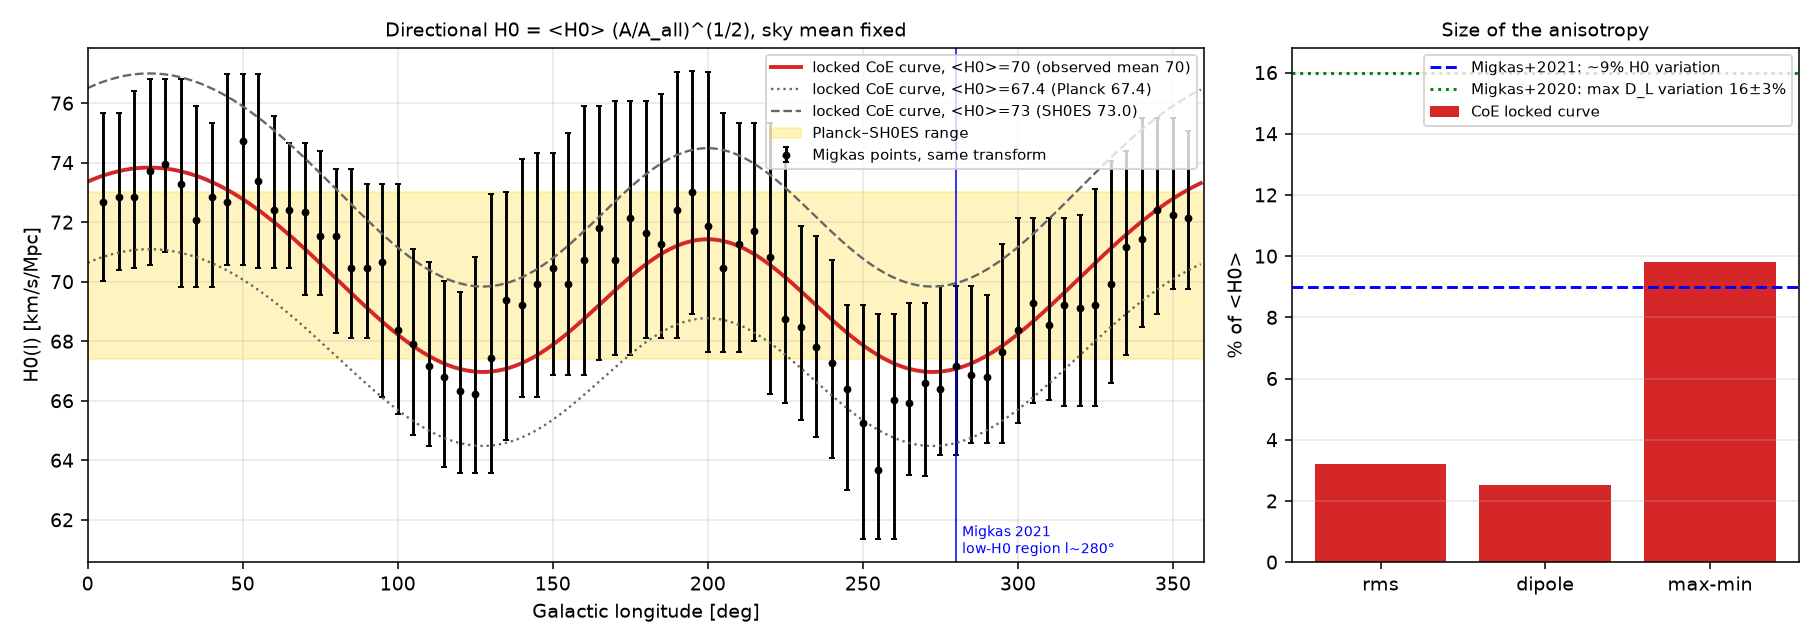
\includegraphics[width=\textwidth]{N6_H0_direction.png}\caption{\NEW Directional $H_0(l)=70\,(A/A_{\rm all})^{1/2}/\langle(A/A_{\rm all})^{1/2}\rangle$ from the locked CoE fit (red, sky mean fixed to the observed 70), with the same curve for means 67.4 (Planck, dotted) and 73.0 (SH0ES, dashed); yellow band: Planck--SH0ES range; points: Migkas et al.\ (2020) cones with the same transform. The Planck and SH0ES curves bracket the Migkas error bars. Fit in $H_0$ space: $r^2=0.744$, $\chi^2=9.06$ (71 cones, correlated, descriptive) vs 44.5 for flat 70. Right: rms, dipole and peak-to-peak of the curve against Migkas et al.\ (2021, $\sim9$\,\%) and (2020, $16\pm3$\,\% in $D_L$). Scripts: \texttt{N6\_H0\_direction.py}, \texttt{N6\_H0\_r2.py}.}\label{fig:H0dir}\end{figure*}



\subsection{Correlated bins and model comparison for the cluster profile}\label{sec:cov}
Adjacent cones share most of their clusters. If clusters are roughly uniform in longitude, two $90^\circ$ cones separated by $\Delta l$ share a fraction
\begin{equation}
\rho(\Delta l)=\max\!\left(0,\,1-\frac{|\Delta l|}{90^\circ}\right)\label{eq:rho}
\end{equation}
of their clusters (circular in $l$). We take this as the correlation matrix and scale it by the errors. The $71\times71$ matrix is nearly singular, so we use its pseudo-inverse keeping eigenvalues above 1\,\% of the largest (15 modes). The effective number of independent bins, $n_{\rm eff}=(\mathrm{tr}\,C)^2/\mathrm{tr}\,C^2$, is 5.98.

\begin{table}[!htb]\centering\small\caption{Migkas $A/A_{\rm all}$: independent-error and overlap-covariance $\chi^2$, $k$ fitted parameters. $p$-values are for $\Delta\chi^2_C$ against isotropy with $k$ degrees of freedom. Source: \texttt{N2\_migkas\_cov.json}.}\label{tab:cov}
\begin{tabular}{@{}lrrrrrr@{}}\toprule
model & $k$ & $\chi^2_{\rm indep}$ & $\chi^2_C$ & $\Delta\chi^2_C$ vs iso & $p$ & BIC$_C$\\\midrule
isotropy & 0 & 45.14 & 8.99 & -- & -- & --\\
free dipole & 3 & 29.36 & 6.90 & 2.09 & 0.55 & 12.26\\
dipole + quadrupole & 5 & 10.86 & 5.20 & 3.79 & 0.58 & 14.14\\
CoE, $D=34.96$ ($D,\eta,m_c,l_0$) & 4 & 9.25 & 3.88 & 5.11 & 0.28 & 11.04\\\bottomrule
\end{tabular}\end{table}

\paragraph{Reading.} The ordering is the same with and without the covariance: the CoE geometry gives the lowest $\chi^2$ with fewer parameters than a dipole + quadrupole, and the lowest BIC. But the improvements over isotropy are not significant ($p=0.28$--0.58) once the bins are correlated, because the 71 cones carry about six independent numbers. The cluster result is therefore qualitative: the off-centre geometry produces the two-hump shape in the right places, with an amplitude tied to CatWISE, but these data alone cannot reject isotropy. The covariance model (Eq.~\ref{eq:rho}) is an approximation. \todo{TO COMPUTE: bootstrap covariance from the 313-cluster catalogue.}

\FIG{N2_migkas_cov.png}{1.0}{\NEW Left: Migkas $A/A_{\rm all}$ with isotropy, a free dipole ($k=3$), a dipole + quadrupole ($k=5$) and the CoE profile at $D=34.96$\,Gpc ($k=4$). Right: independent-error and overlap-covariance $\chi^2$ for each ($n_{\rm eff}=6.0$). Script: \texttt{N2\_migkas\_cov.py}.}{fig:cov}

\paragraph{$B/B_{\rm all}$.} $B$ is not refitted on the rev7 background and is not claimed.

\subsection{The CMB: the deterministic sky at last scattering}\label{sec:cmb}
Carried to last scattering at $R=R_{\rm ls}=0.18957$\,Gpc on the rev7 background, the smooth CoE sky (the background map of the famP solution at $D=34.96$\,Gpc) has rms $\Delta T/T=2.32\times10^{-5}$. Its multipole amplitudes are $2.18\times10^{-5}$ at $\ell=1$, $9.3\times10^{-8}$ at $\ell=2$, $7.7\times10^{-6}$ at $\ell=3$, and below $1.4\times10^{-7}$ for $\ell=4$--5. At the consistent, much smaller $R_{\rm ls}$, the deterministic sky is already at the $10^{-5}$ level, dominated by the dipole and octupole.

\subsection{Compensating structure inside the last-scattering sphere}\label{sec:comp}
The question of \S\ref{sec:intro} is whether some physically allowed set of masses can make that sky as flat as observed. We place 3,000 point bodies (seed 2000) at $0.075R<r<0.875R$ from the observer, softened at $0.025R$, each with $|M|\le10^{14}\,M_\odot$, and solve a bounded least-squares problem for their masses. The target is to cancel the background at $\ell=1$--12, while penalising $\ell=13$--40, and to cancel a fraction $1-f=0.74$ of the stochastic field's own $\ell=2$ on the seed-42 sky, so that the observed $D_2$ is approached.

\paragraph{Result} (\texttt{p5\_c\_p8}). 975 clusters ($M_+=2.98\times10^{15}M_\odot$) and 904 voids ($M_-=-3.25\times10^{15}M_\odot$), counting bodies above threshold. No body sits at the mass bound. The residual sky has rms $5.67\times10^{-6}$ and maximum $1.27\times10^{-5}$. Its dipole is $3.9\times10^{-11}$ and its octupole $1.1\times10^{-9}$.
The relevant error is not the residual itself but the residual against the target. With $F_{\rm target}$ the $\ell=2$ part of the field map scaled by $(1-f)$, the maximum of $|{\rm Resid}+F_{\rm target}|$ over the sky is $1.50\times10^{-6}$ (rms $3.2\times10^{-7}$), below the $10^{-5}$ goal. The $\ell=2$ part of that error is $8.3\times10^{-10}$ (\texttt{p5\_err.py}). On the seed-42 sky, $D_2$ falls from 1,042.3 to 70.49\,$\mu$K$^2$ (target 70.46).
\paragraph{Cluster sky unchanged.} The bodies perturb the cluster lines of sight by $\Delta\Phi/c^2=2.8$--$4.3\times10^{-9}$. The Migkas $\chi^2$ moves from 9.278230532 to 9.278230704 ($r^2=0.74805$ unchanged, $\max|\Delta A|=1.9\times10^{-9}$).

\FIG{d2_web.png}{1.0}{\NEW The compensating bodies of the final run (\texttt{p5\_c\_p8}). Left: mass histogram of clusters and voids. Middle: mass against distance from the observer in units of $R$. Right: the bodies-only sky $\Delta T/T$. Script: \texttt{d2\_web.py}.}{fig:web}

\why{The bodies are Newtonian point masses with tidal-shear sky kernels inside a sphere of radius 0.19\,Gpc. Their total masses are $\sim3\times10^{15}M_\odot$ of each sign, comparable to a few rich clusters. Whether such a configuration forms naturally is not addressed, and a configuration solved for to cancel the dipole is, by construction, fine-tuned. It shows existence, not likelihood.}

\subsection{Stochastic field and sky projection}\label{sec:field}
The density contrast is a zero-mean Gaussian random field with power $P_\delta(k)$, and $\Phi_k=-(4\pi G\bar\rho/k^2)\delta_k$. A photon crossing it picks up the Sachs--Wolfe, integrated Sachs--Wolfe and moving-lens terms. The moving lens supplies almost all of the power. Confined to a radial window $W(\chi)=\exp[-(\chi-\chi_w)^2/2s_w^2]$, the exact projection is
\begin{equation}
C_\ell=\frac{2}{\pi}\int k^2dk\,P_\Phi(k)|\Delta_\ell(k)|^2,\qquad \Delta_\ell(k)=\int d\chi\,KWj_\ell(k\chi),\label{eq:exact}
\end{equation}
used for $\ell\le50$, and the Limber form
\begin{equation}
D_\ell\simeq\frac{\ell(\ell+1)T_0^2}{2\pi}\int d\chi\,\frac{[K_MW]^2}{\chi^2}\,\frac{k^2}{3}P_\Phi(k)\Big|_{k=\nu/\chi},\quad \nu=\ell+\tfrac12,\label{eq:limber}
\end{equation}
is corrected by $c_\ell=C^{\rm exact}_\ell/C^{\rm Limber}_\ell$ above $\ell=50$.

\paragraph{Changes on the rev7 background.} The moving-lens velocity factor uses $D=34.96$\,Gpc and the source shell $R=R_{\rm ls}=0.18957$\,Gpc. $D^{\rm fix}_\ell$ is the low-$\ell$ ($\ell\le40$) spectrum of the compensated sky of \S\ref{sec:comp}.

\paragraph{Source spectrum.} The fitted form, with $K_0=100/s$ and $k$ in Gpc$^{-1}$, is
\begin{equation}
P_\delta=10^{\lg A}k^{\,n+\alpha\ln(k/K_0)}\Big[1+A_w\Big(\tfrac{k}{K_0}\Big)^{\beta}\cos(kr_s+\phi)+Be^{-k/k_B}\cos(kr_2+\phi_2)\Big]e^{-(k/k_D)^m}.\label{eq:Pk}
\end{equation}
The oscillatory terms are phenomenological and fitted. They describe the acoustic peaks; they do not derive them. With $\alpha=\beta=0$ and $m=2$ the form reduces to a 12-parameter model. The 15 parameters were fitted by a multistart Nelder--Mead search (12 starts) of the fit objective, with the exact/Limber correction refreshed between passes (correlation of successive $c_\ell$ 0.899 then 0.978). Best fit: $\lg A=-10.508$, $n=0.298$, $\alpha=-0.00365$, $A_w=0.297$, $\beta=-0.00666$, $r_s=0.003732$\,Gpc, $\phi=1.414$, $k_D=4104$\,Gpc$^{-1}$, $m=1.250$, $\chi_w=0.1724$\,Gpc, $s_w=0.01096$\,Gpc, $B=0.734$, $k_B=3343$\,Gpc$^{-1}$, $r_2=0.00188$\,Gpc, $\phi_2=4.054$. Note $r_2\approx r_s/2$ and $\chi_w=0.91R$.
\paragraph{Peak spacing.} An oscillation $\cos(kr_s)$ gives peaks spaced by $\Delta\ell\approx2\pi\chi_{\rm eff}/r_s$. With $r_s=0.003732$\,Gpc and $\chi_{\rm eff}\approx\chi_w=0.1724$\,Gpc, $\Delta\ell\approx290$, close to the spacing of the model peaks in Table~\ref{tab:tt}.
\paragraph{No parameter uncertainties.} Nelder--Mead returns a point. \todo{TO COMPUTE: Hessian or MCMC widths at the optimum.}

\subsection{$TT$ fit}\label{sec:tt}
\begin{table}[!htb]\centering\small\caption{$TT$ statistics of the current solve (p8 field on the rev7 background, with the compensating bodies). $\Delta$ values are against $\Lambda$CDM with $N=2499$, $p=15$ vs 6. Sources: \texttt{p6\_p8.json}, \texttt{N4\_tt\_stats.json}.}\label{tab:tt}
\begin{tabular}{@{}lrrrrrr@{}}\toprule
 & $\chi^2_{2-30}$ & $\chi^2_{30-2500}$ & $\chi^2_{2-2500}$ & $r^2_{2-2500}$ & $\Delta\chi^2$ & $\Delta$BIC\\\midrule
$\Lambda$CDM (Planck best fit) & 20.14 & 2538.39 & 2558.49 & 0.983 & -- & --\\
CoE ensemble mean & 29.33 & 2586.91 & 2616.19 & 0.982 & +57.7 & +128.1\\
CoE seed 42 & 32.76 & 3308.41 & 3340.22 & -- & +781.7 & +852.1\\
CoE seed 42, compensated $\ell\le40$ & 31.38 & 3308.17 & 3338.67 & 0.975 & +780.2 & +850.6\\\bottomrule
\end{tabular}\end{table}

\noindent Fit objective (low-$\ell$ unbinned + binned, the minimised quantity): CoE 141.78, $\Lambda$CDM 98.75. Peaks, with one finder for all three spectra (Savitzky--Golay 61/3, prominence 20, separation $\ge200$): Planck 224, 514, 822, 1124, 1405; CoE 221, 536, 814, 1126, 1417; $\Lambda$CDM 220, 536, 813, 1127, 1421.

\paragraph{Reading.} On the consistent background the ensemble mean comes within $\Delta\chi^2=+58$ of $\Lambda$CDM over $\ell=2$--2500 . Because $p$ is larger, $\Delta$BIC is $+128$, so $\Lambda$CDM is still strongly preferred. The model peak positions agree with $\Lambda$CDM's to within 1--4 in $\ell$; on unbinned data the smoothed Planck second peak (514) is pulled by noise, so the peak list is descriptive. The seed-42 numbers are one draw. Section~\ref{sec:seeds} puts them in context.

\FIG{d3_stoch.png}{1.0}{\REGEN $TT$ spectrum of the current solve against Planck 2018 and $\Lambda$CDM, with residual panel. Models are drawn above the data. Ensemble mean $\chi^2_{2-2500}=2{,}616$; compensated seed-42 sky 3,339; $\Lambda$CDM 2,558. Script: \texttt{d3\_stoch.py}.}{fig:tt}

\subsection{Distribution of skies}\label{sec:seeds}
The path-dependence argument of \S\ref{sec:intro} makes the distribution of one-sky $\chi^2$ the relevant statistic. We draw 1,000 skies as $D_\ell=D^{\rm fix}_\ell+D^{\rm field}_\ell\chi^2_{2\ell+1}/(2\ell+1)$ and, for a like-for-like comparison, 1,000 $\Lambda$CDM skies the same way. Planck's errors already include cosmic variance, so absolute one-sky $\chi^2$ values double-count it for both models. Only the comparison between the two distributions is meaningful.

Results (\texttt{N5\_seed\_distribution.json}). Over $\ell=2$--2500 the CoE median is 3,347 (16--84\,\%: 3,286--3,408), against 3,279 (3,221--3,338) for $\Lambda$CDM. Over $\ell=2$--30 the CoE median is 50.1 (39.3--63.8), against 42.4 (32.0--55.8). Seed 42 (3,340; 32.8) is typical of the model distribution. Of the CoE skies, 26\,\% pass a strict 5\,\% consistency cut at low $\ell$ ($\chi^2_{2-30}<43$), and 99.3\,\% pass a loose cut ($<100$). This answers the pass-rate question (referee M9) for the current field.

\FIG{N5_seed_distribution.png}{1.0}{\NEW One-sky $\chi^2$ over 1,000 realisations of the current CoE field (grey) and of $\Lambda$CDM drawn the same way (black outline), for $\ell=2$--30 (left) and 2--2500 (right). Vertical lines: $\Lambda$CDM mean curve, seed 42, CoE median. Script: \texttt{N5\_seed\_distribution.py}.}{fig:seeds}

\subsection{Joint summary}\label{sec:joint}
Figure~\ref{fig:joint} collects the pieces of the solve on the one background.

\FIG{N3_joint_summary.png}{1.0}{\NEW Joint summary of the rev7 solve ($D=34.96$\,Gpc, $R=0.18957$\,Gpc). Top: deterministic background sky (rms $2.32\times10^{-5}$); residual after a background-only compensation run (bodies at $R$, $f=1$; rms $3.2\times10^{-7}$). Middle: rms per $\ell$ before and after that run; Migkas $\chi^2$ against $D$. Bottom: low-$\ell$ and full $TT$ spectra of the final run (p8 field, \texttt{p5\_c\_p8} bodies) with $\Lambda$CDM and Planck. Script: \texttt{N3\_joint\_summary.py}.}{fig:joint}

\subsection{Open CMB problems}\label{sec:open}
\paragraph{1. Which velocity.} The moving-lens kernel uses the CoE radial velocity of the matter. In a Newtonian picture, a velocity common to observer, lens and source produces no anisotropy; only the velocity relative to the observer, $\vec V_H=\vec V_g-\vec V_O$, should enter. Near the observer $\vec V_H\approx H\chi\hat n$ is nearly radial, and a radial velocity contributes little to the transverse (Limber) signal. On the rev7 background $R_{\rm ls}=0.19$\,Gpc and $V_H\lesssim HR\approx0.02c$, against $V_O\approx4c$, so the relative-velocity kernel would be about two orders of magnitude weaker in amplitude. The amplitude $\lg A$ would absorb a uniform rescaling, but the shape would change. \todo{TO COMPUTE: refit with the relative-velocity kernel.}
\paragraph{2. Statistical anisotropy.} With $\vec u$ along a fixed axis, the local small-scale power varies as $1-\cos^2\theta=\tfrac23[1-P_2(\cos\theta)]$: a 100\,\% quadrupolar modulation that vanishes along the CoE axis and is hidden by the orientation average $\langle(\hat k\cdot\hat u)^2\rangle=1/3$. Planck constrains such modulations at the percent level (Planck Collaboration 2020b). If the relative velocity is used instead, the modulation changes. \todo{TO COMPUTE: predicted modulation and comparison with Planck.}
\paragraph{3. Polarisation.} $TE$ and $EE$ are not computed. They are the natural held-out test (\S\ref{sec:disc}).

\subsection{Sky anomalies}\label{sec:anom}
No anomaly score is claimed in this revision: the residual sky maps have not been rebuilt on the rev7 background (the earlier analysis and the audit of it are in Appendix~\ref{app:superseded}). \todo{TO COMPUTE: rotation and isotropic-mock null with the rev7 profile, pairs collapsed.}

\subsection{Supporting figures recomputed on the rev7 background}\label{sec:rev7figs}
Every figure in this subsection was recomputed from the rev7 solve products at $D=34.96$\,Gpc, $R=R_{\rm ls}=0.18957$\,Gpc (scripts named in each caption, \texttt{.py} beside each PNG). They document the modulation, the direct fits, the bodies, the kernel and target construction, the source window, the low-$\ell$ spectrum, the stage-A fit, the one-sky spread, the shell ladder, the parameter degeneracies and the damped-harmonic residual of the rev7 field fit. The rev6 prose that originally accompanied them used the earlier backgrounds and is kept only in Appendix~\ref{app:superseded}.
\FIGc{R16_mod.png}{0.32}{\textbf{[REGEN rev7: \texttt{R16\_mod.py}; recomputed at $D=34.96$\,Gpc]}\ CoE modulation $m(r)=\exp\sum_kc_k(\min(r/D,R_b)-1)^{k+1}$, $c=[-0.041,-0.035,0.1353,0]$ (the same law and $c_k$ used in the rev7 ray trace), $R_b=1.5(1+R_V/D)$, $R_V=14.30$\,Gpc. At $D=34.96$\,Gpc: slope at the observer $-1.17\times10^{-3}$\,Gpc$^{-1}$ (cf.\ CatWISE-locked $\rho'/\rho\approx-0.00106$), $m=1.0017$ and $0.9867$ at the near and far edges of the gold observable band $D\pm R_V=20.7$--$49.3$\,Gpc. Grey: beyond the observable edge, unconstrained; nothing drawn. Axis cut at 80\,Gpc.}{r6:fig:mod}
\FIGc{R06_direct_fits.png}{0.3}{\textbf{[REGEN rev7: \texttt{R06\_direct\_fits.py}; recomputed from the rev7 solve products.]}\ (1) Migkas $A/A_{\rm all}$ (71 cones) with the profile refit at $D=30$, 34.96, 42, 50, 58.2\,Gpc ($\chi^2=9.53$, 9.25, 9.59, 10.28, 10.89; $D=34.96$ bold). (2) Ray-traced background CMB $\Delta T/T$ vs angle from the CoE direction (\texttt{p2\_trace}, monopole removed) at $D=34.96$, 42, 58.2. (3) Initial density shape vs $r/D$ (same $c_k$, $R_b$ depends on $D$). (4) Background-sky $D_\ell$, $\ell=2$--6, against Planck: before the bodies, $\ell=3$ is $\approx1500\,\mu$K$^2$, which the bodies remove (\S CMB). The two humps come from $\cos\psi(l)$ at fixed galactic latitude.}{r6:fig:mig}
\FIGc{R11_web.png}{0.62}{\textbf{[REGEN rev7: \texttt{R11\_web.py}; recomputed on the rev7 solve.]}\ The web actually used by the rev7 CMB solve: the 3000 bodies of \texttt{p5\_c\_p8.npz} (1575 clusters, 1425 voids, all inside $R_{\rm ls}=0.18957$\,Gpc). Left: slab $|z|<0.02$\,Gpc, marker size $\propto|M|^{1/2}$; dashed: $R_{\rm ls}$. Middle: zoom. Right: number density of clusters and voids vs radius.}{r6:fig:web}
\begin{figure*}[t]\centering\fig{\textwidth}{0.3\textheight}{R12_ladder.png}\caption{\textbf{[REGEN rev7: \texttt{R12\_ladder.py}; kernels $\sigma_s=0.005$--$0.08$\,Gpc inside the $R_{\rm ls}=0.19$\,Gpc sphere]}\ Smoothing ladder of the rev7 bodies: signed mass deposited on a $128^3$ grid over $R_{\rm ls}$ and Gaussian-smoothed; slab $z=0$. Right: rms signed density vs kernel.}\label{r6:fig:ladder}\end{figure*}
\FIGc{R10_harmonics.png}{0.5}{\textbf{[REGEN rev7: \texttt{R10\_harmonics.py}; pure geometry, no $D$ or $R$ enters]}\ Single axisymmetric harmonics $\ell=0\ldots7$ drawn as density on a ring of 400 bodies (blue over-, orange under-density). Bars: power measured from the bodies by Legendre projection (not set by hand).}{r6:fig:h1}
\begin{figure*}[t]\centering\fig{\textwidth}{0.5\textheight}{R13_target_profiles.png}\caption{\textbf{[REGEN rev7: remade from the caption's method, \texttt{R13\_target\_profiles.py} (original script not found); dimensionless in $R$, so independent of $D$]}\ Target profiles matched numerically: a fixed mass at $1.55R$ plus 40 fitted axisymmetric clump/void rings (ridge least squares) reproduce $\cos(\theta/2)$, $\cos1.5\theta$, $\cos2.5\theta$, $\cos2\theta$ with $R^2>0.9999$ (top: target, fit, fixed mass alone; bottom: fitted rings).}\label{r6:fig:inv}\end{figure*}
\begin{figure*}[t]\centering\fig{\textwidth}{0.5\textheight}{R14_inverse_ell220.png}\caption{\textbf{[REGEN rev7: Chris's original inverse-design code re-run unchanged (\texttt{R14\_inverse\_ell220.py}, from \texttt{book/recovered/f13.py}); dimensionless in $R$ (shell at $1.012R_{\rm ls}$)]}\ Target peak matched numerically: a non-axisymmetric source shell at $r=1.012R$ (gravitational potential, not temperature) built from 3D clumps/voids reproduces a prescribed peak at $\ell=220$ with widths $\sigma_\ell=32$ and 8.}\label{r6:fig:inv2}\end{figure*}
\FIGc{R18_pdelta_window.png}{0.29}{\REGEN from the rev7 field fit (\texttt{p8}): $\chi_w=0.1724$, $s_w=0.0110$\,Gpc, $R=0.18957$\,Gpc. Script \texttt{R18\_pdelta\_window.py}. Fitted $P_\delta$ split into its terms (left) and the radial window $W(\chi)$ (right).}{r6:fig:pdelta}
\FIGc{R21_lowell.png}{0.3}{\REGEN from the rev7 solve (\texttt{p6\_p8}); script \texttt{R21\_lowell.py}. Low multipoles (linear axes), $\ell=2$--30: $\Lambda$CDM (black), Planck (grey points), CoE ensemble mean (red), CoE one-sky realisation (seed 42 with compensating bodies, magenta dashed).}{r6:fig:low}
\FIGc{R17_stageA.png}{0.3}{\textbf{[REGEN rev7: \texttt{R17\_stageA.py}; recomputed on the rev7 field. The p8 fit is an unregularised multistart, so there is no $\lambda$]}\ Low-$\ell$ fit, $\ell$ 2--30, rev7 background ($D=34.96$\,Gpc, $R_{\rm ls}=0.18957$\,Gpc). Blue: ensemble mean $D_{\rm fix}+D_f$ with $\pm1\sigma$ cosmic-variance band ($\chi^2_{\rm Planck+CV}=16.4$, $\chi^2_{\rm Planck}=29.3$, Pearson $r^2=0.001$); red dashed: deterministic part $D_{\rm fix}$ (negligible at these $\ell$); black: ΛCDM ($\chi^2_{\rm Planck}=20.1$, $r^2=0.012$); points: Planck 2018.}{r6:fig:ac}
\FIGc{R20_pass.png}{0.6}{\textbf{[REGEN rev7: \texttt{R20\_pass.py}. $R=R_{\rm ls}=\eta_{\rm rec}D$ is fixed by the background; one-sky spread at that $R$]}\ 1000 one-sky realisations of the p8 field (generator and seed as Fig.~\ref{fig:seeds}), $\ell$ 2--30. Left: 16--84\% bands of all skies, of the 993 passing the loose cut ($\chi^2<100$) and the 261 passing the strict cut ($\chi^2<43$), with ΛCDM and Planck. Right: distribution of one-sky $\chi^2$ (median 50.1).}{r6:fig:pass}
\FIGc{R22_ladder.png}{0.28}{\textbf{[REGEN rev7: \texttt{R22\_ladder.py}; recomputed on the rev7 field. Shell at $R=0.8$, 1.0, $1.2\,R_{\rm ls}$ with the window kept at the same depth]}\ The same p8 source parameters with the shell at $R=0.152$, 0.190, 0.227\,Gpc: peaks at $\ell=[175,425,644]$, $[221,536,814,1126]$, $[267,648,985,1360]$; fit statistic $1.07\times10^5$, 141.8, $1.50\times10^5$. Peak positions scale with $R$; only $R=R_{\rm ls}$ fits.}{r6:fig:acl}
\begin{figure*}[b]\centering\fig{\textwidth}{0.3\textheight}{R23_degeneracy.png}\caption{\textbf{[REGEN rev7: \texttt{R23\_degeneracy.py}; recomputed on the rev7 p8 field fit]}\ Parameter degeneracies of the rev7 fit, $22\times21$ and $21\times21$ grids, the other 13 parameters held at the best fit (star, statistic 141.8). Left: window centre $\chi_w$ vs amplitude $\lg A$. Right: $P_\delta$ slope $n$ vs $\lg A$. Colour: $\log_{10}$ of the fit statistic; contours $\Delta\chi^2=2.3,6.2,11.8$. These are slices, not marginalised uncertainties.}\label{r6:fig:deg}\end{figure*}
\begin{figure*}[t]\centering\fig{\textwidth}{0.62\textheight}{R19_damped_harm.png}\caption{\textbf{[REGEN rev7: \texttt{R19\_damped\_harm.py}; refitted to the rev7 residual]}\ Damped-harmonic fits (Eqs.~\ref{r6:eq22}--\ref{r6:eq23}) to $\epsilon_\ell=(D^{\rm Planck}_\ell-D^{\rm CoE}_\ell)/\sigma_\ell$ of the rev7 ensemble mean, with 7, 8, 9 harmonics (best $\Delta\ell\approx840$--850, $L=2250$--3000), and Pearson $r^2$ versus number of harmonics (bottom). Result: $r^2\le0.022$ for every model; the rev7 residual has no coherent harmonic structure, unlike the rev6 residual ($\Delta\ell=593$, $L=990$).}\label{r6:fig:damp}\end{figure*}
\clearpage

\section{Discussion}\label{sec:disc}
\paragraph{What is fitted and what is predicted.} Predicted before the data: the two-hump shape, ring locations, the sign of the gradient (Table~\ref{tab:pred}). Fitted: $D$, $\eta$, $m_c$, $l_0$; $L$ by the lock; the masses of the compensating bodies; the 15 source-spectrum parameters. Appendix~A counts them.

\paragraph{Cluster sky.} A single off-centre axis with a CatWISE-locked gradient reproduces the two-hump shape of $A/A_{\rm all}$ with fewer parameters than a dipole + quadrupole and with the lowest BIC, but with about six independent bins no model is significantly preferred over isotropy. The direction is right; the significance is qualitative.

\paragraph{CMB.} On one background, a physically bounded set of bodies cancels the deterministic dipole and octupole below $10^{-9}$, reaches the $D_2$ target within $1.5\times10^{-6}$, and leaves the cluster fit untouched. The stochastic field brings the ensemble-mean $TT$ fit to within $\Delta\chi^2=+58$ of $\Lambda$CDM. However, $\Delta$BIC $=+128$ and the like-for-like realisation medians differ by $\approx70$, so $\Lambda$CDM fits better. The acoustic peaks are put in through $P_\delta$, and the moving-lens velocity frame may change the result qualitatively.

\paragraph{Off-centre bounds.} Alnes \& Amarzguioui (2006) and Foreman et al.\ (2010) bound an off-centre observer in a void by the CMB dipole and quadrupole \emph{without} compensating structure. Here the dipole is removed by structure inside $R_{\rm ls}$. This is a loophole only if that structure is plausible. A solved-for configuration is fine-tuned by construction, so the bound is not evaded in any probabilistic sense.

\paragraph{Internal consistency.} The paper uses one distance ($D=34.96$\,Gpc), one background (LTB famP), and one axis ($l_0=19.87^\circ$). Remaining tensions: $H_0=34.3$ and $t_0=0.314$\,Gyr against observed values (setting $D=17.1$\,Gpc for $H_0=70$ degrades Migkas to $r^2=0.49$, Table~\ref{tab:Dscan}), and the profile-core age (2.78\,Gyr) against the LTB age.

\paragraph{Limits.}
\begin{itemize}
\item The thermal history at recombination is FRW-like by assumption.
\item The moving lens is a Newtonian-gauge kernel on an LTB background, with the velocity frame open.
\item The cluster covariance is a geometric approximation, not a bootstrap.
\item The CatWISE lock ignores the kinematic dipole, bias and the redshift kernel, and samples radii beyond $R_{\rm ls}$.
\item No parameter uncertainties are given for the 15-parameter source spectrum.
\item Whether an off-centre observer would infer apparent acceleration from supernova distances has not been computed.
\end{itemize}

\paragraph{Next steps, in priority order.}
\begin{enumerate}
\item Refit the field with the relative-velocity moving-lens kernel; compute the quadrupolar modulation and compare with Planck.
\item Find an LTB family that keeps the cluster and CMB results with $H_0$ and $t_0$ nearer observed values.
\item Redo the CatWISE lock with the kinematic-subtracted dipole and the CatWISE $dN/dz$ on the LTB distance--redshift relation.
\item Bootstrap the Migkas covariance from the 313-cluster catalogue.
\item Held-out tests: predict $TE/EE$; fit $\ell\le1200$ and predict $\ell>1200$; fit $A$ and predict $B$.
\item Rebuild the anomaly maps on the rev7 profile with a rotation null.
\item Compute $D_L(z,\hat n)$ along off-centre lines of sight against Pantheon+.
\end{enumerate}

\section{Conclusions}\label{sec:concl}
\begin{enumerate}
\item The toy universe now runs on one background: an LTB solution with the observer at $D=34.96$\,Gpc, giving $H_0=34.3$\,km\,s$^{-1}$\,Mpc$^{-1}$, age 0.314\,Gyr and $R_{\rm ls}=0.190$\,Gpc. Those values are a tension of the model, stated rather than hidden. With the sky mean fixed by observation at $\langle H_0\rangle=70$, the locked fit gives a directional $H_0(l)$ with $r^2=0.744$ ($\chi^2=9.06$ vs 44.5 for flat 70), range 66.97--73.83 and 9.8\,\% peak to peak, bracketed by the Planck and SH0ES values (Fig.~\ref{fig:H0dir}).
\item On the cluster sky the off-centre geometry goes the right way. It gives the lowest $\chi^2$ and BIC among isotropy, dipole, dipole + quadrupole and CoE under an approximate covariance. With about six effective bins, the preference is qualitative.
\item On the CMB, a bounded set of 975 clusters and 904 voids inside the last-scattering sphere flattens the deterministic CoE sky to the target within $1.5\times10^{-6}$ without disturbing the cluster fit. With a phenomenological source spectrum, the $TT$ ensemble mean comes within $\Delta\chi^2=+58$ of $\Lambda$CDM, while $\Delta{\rm BIC}=+128$ still favours $\Lambda$CDM.
\item The decisive open problems are the moving-lens velocity frame and the quadrupolar modulation it implies, a realistic $H_0$ and age, and a held-out prediction.
\end{enumerate}

\section*{References}\addcontentsline{toc}{section}{References}
\small Please verify volume and page numbers before circulation.
\begin{itemize}\itemsep0pt
\item Alnes, H., \& Amarzguioui, M. (2006). CMB anisotropies seen by an off-center observer in a spherically symmetric inhomogeneous universe. Phys.\ Rev.\ D 74, 103520.
\item Birkinshaw, M., \& Gull, S.\,F. (1983). A test for transverse motions of clusters of galaxies. Nature 302, 315.
\item Biswas, T., Notari, A., \& Valkenburg, W. (2010). Testing the void against cosmological data. JCAP 11, 030.
\item Box, G.\,E.\,P. (1976). Science and statistics. J.\ Am.\ Stat.\ Assoc.\ 71, 791.
\item Clarkson, C., Bassett, B., \& Lu, T.\,H.-C. (2008). A general test of the Copernican principle. Phys.\ Rev.\ Lett.\ 101, 011301.
\item Eisenstein, D.\,J., \& Hu, W. (1998). Baryonic features in the matter transfer function. ApJ 496, 605.
\item Ellis, G.\,F.\,R., \& Stoeger, W.\,R. (1987). The `fitting problem' in cosmology. Class.\ Quantum Grav.\ 4, 1697.
\item Foreman, S., Moss, A., Zibin, J.\,P., \& Scott, D. (2010). Spatial and temporal tuning in void models for acceleration. Phys.\ Rev.\ D 82, 103532.
\item Garc\'ia-Bellido, J., \& Haugb{\o}lle, T. (2008). Looking the void in the eyes --- the kinematic Sunyaev--Zeldovich effect in LTB models. JCAP 09, 016.
\item Mayo, D.\,G. (1996). Error and the Growth of Experimental Knowledge. University of Chicago Press.
\item Migkas, K., Schellenberger, G., Reiprich, T.\,H., et al.\ (2020). Probing cosmic isotropy with a new X-ray galaxy cluster sample through the $L_X$--$T$ scaling relation. A\&A 636, A15.
\item Migkas, K., Pacaud, F., Schellenberger, G., et al.\ (2021). Cosmological implications of the anisotropy of ten galaxy cluster scaling relations. A\&A 649, A151.
\item Moss, A., Zibin, J.\,P., \& Scott, D. (2011). Precision cosmology defeats void models for acceleration. Phys.\ Rev.\ D 83, 103515.
\item Press, W.\,H., \& Schechter, P. (1974). Formation of galaxies and clusters of galaxies by self-similar gravitational condensation. ApJ 187, 425.
\item Planck Collaboration (2020a). Planck 2018 results. V. CMB power spectra and likelihoods. A\&A 641, A5.
\item Planck Collaboration (2020b). Planck 2018 results. VII. Isotropy and statistics of the CMB. A\&A 641, A7.
\item Secrest, N.\,J., von Hausegger, S., Rameez, M., et al.\ (2021). A test of the cosmological principle with quasars. ApJL 908, L51.
\item Sheth, R.\,K., \& van de Weygaert, R. (2004). A hierarchy of voids: much ado about nothing. MNRAS 350, 517.
\item Tukey, J.\,W. (1977). Exploratory Data Analysis. Addison-Wesley.
\item Zhang, P., \& Stebbins, A. (2011). Confirmation of the Copernican principle at Gpc radial scale and above from the kinetic Sunyaev--Zel'dovich effect power spectrum. Phys.\ Rev.\ Lett.\ 107, 041301.
\end{itemize}
\normalsize
\appendix
\section{Parameter accounting}
\begin{table}[H]\centering\small
\begin{tabular}{@{}p{4.2cm}p{7.4cm}p{3.2cm}@{}}\toprule
Claim & Quantities chosen with the data in view & $p$ (approx.)\\\midrule
Migkas $A/A_{\rm all}$ (\S\ref{sec:laws}) & $D$, $\eta$, $m_c$, $l_0$; $L$ by the lock; law family (1 of 7) & 4 continuous + 1 discrete\\
Choice of $D$ (Fig.~\ref{fig:Dprof}) & profile minimum over 5 values & included above\\
CatWISE lock & $d=14.3005$\,Gpc, $\delta=0.031$ (assumed) & 0 fitted, 2 assumed\\
Background (\S\ref{sec:bg}) & LTB famP family; $D$ from the cluster fit & 1 discrete\\
Compensating bodies (\S\ref{sec:comp}) & 3,000 masses (bounded LSQ), positions seeded (2000); $\ell_{\rm max}=12$, $\lambda=10^{-5}$, $f=0.26$ & solved, not fitted to $TT$; $f$ 1\\
$TT$ field (\S\ref{sec:field}) & $\lg A,n,\alpha,A_w,\beta,r_s,\phi,k_D,m,\chi_w,s_w,B,k_B,r_2,\phi_2$ & 15\\
$TT$ structural choices & acoustic term; damped term (period first read off a residual in rev5); running and tilt terms added in rev7 & $\ge3$ discrete\\
Anomaly score & withdrawn in rev7 & --\\\bottomrule
\end{tabular}\end{table}

\section{Figure provenance}
Every rev6 figure is kept (entries marked App.~\ref{app:superseded} are in the superseded appendix; the rest are in the body), and every figure in the draft now has a \texttt{.py} in \texttt{fig7/} that makes it, except the hand-drawn preprint sketch (rev6 Fig.~1 top and middle), which stays as an image. \texttt{R*} scripts read the rev7 solve in \texttt{joint\_solve/phase2/} or are pure geometry; scripts in \texttt{fig7/rerun/} are original rev6 makers re-run unchanged with only the output path redirected. Where no original script was found, the figure was rebuilt from its method (marked ``remade).
\begin{longtable}{@{}lllp{6.2cm}@{}}\toprule
rev6 & rev7 & file & status\\\midrule\endhead
1 (bottom) & \ref{fig:setup} & Fig01b\_geometry & updated\\
1 (top, middle) & \ref{fig:setup0} & L01a\_geometry\_top/bot & unchanged: hand-drawn preprint sketch (image, not computed) \textbf{[App.~\ref{app:superseded}]}\\
2 & \ref{fig:vol} & f02\_volume\_time & updated (LTB background)\\
3 & \ref{fig:bg} & d4\_background & updated (LTB replaces rad+matter FRW)\\
4 & \ref{r6:fig:obsAB} & R04\_migkas\_rotation & regenerated: original script re-run (data + spreadsheet model) \textbf{[App.~\ref{app:superseded}]}\\
5 & \ref{fig:laws} & d1\_migkas\_laws & updated ($D=34.96$)\\
6 & \ref{r6:fig:mig} & R06\_direct\_fits & regenerated at $D=34.96$ (rev6 used $D=42$ polynomial runs)\\
7 & \ref{fig:amp} & Fig04\_amp\_full & updated (p7 bodies key fixed)\\
8 & \ref{r6:fig:orient} & R08\_sky\_orientation & regenerated: original maker re-run \textbf{[App.~\ref{app:superseded}]}\\
9 & \ref{r6:fig:overlay} & R09\_overlay\_bands & regenerated: original band code re-run; extrema checked vs rev7 refit \textbf{[App.~\ref{app:superseded}]}\\
10 & \ref{r6:fig:h1} & R10\_harmonics & regenerated: new script, power now measured\\
11 & \ref{r6:fig:web} & R11\_web & regenerated on rev7 bodies (p5\_c\_p8)\\
12 & \ref{r6:fig:ladder} & R12\_ladder & regenerated on rev7 bodies; kernels scaled to $R_{\rm ls}$\\
13 & \ref{r6:fig:inv} & R13\_target\_profiles & remade from method (no original); $D$-independent\\
14 & \ref{r6:fig:inv2} & R14\_inverse\_ell220 & regenerated: original f13 code re-run; $D$-independent\\
15 & \ref{r6:fig:webd} & R15\_web\_ingredients & regenerated from cosmo.py \textbf{[App.~\ref{app:superseded}]}\\
16 & \ref{r6:fig:mod} & R16\_mod & regenerated at $D=34.96$\\
17 & \ref{r6:fig:ac} & R17\_stageA & regenerated on p8 field; L-curve panel not applicable (no $\lambda$)\\
18 & \ref{r6:fig:pdelta} & R18\_pdelta\_window & updated (p8 field)\\
19 & \ref{r6:fig:damp} & R19\_damped\_harm & regenerated on rev7 residual\\
20 & \ref{r6:fig:pass} & R20\_pass & replaced: $R$ scan meaningless ($R=R_{\rm ls}$ fixed); one-sky bands at fixed $R$\\
21 & \ref{r6:fig:low} & R21\_lowell & updated (p6\_p8)\\
22 & \ref{r6:fig:acl} & R22\_ladder & regenerated: $R=0.8,1,1.2\,R_{\rm ls}$\\
23 & \ref{r6:fig:deg} & R23\_degeneracy & regenerated on p8 fit\\
24 & \ref{fig:tt} & d3\_stoch & updated (p6\_p8)\\
25 & \ref{r6:fig:decomp} & R25\_recon\_n3 & regenerated: original script re-run (locked curve) \textbf{[App.~\ref{app:superseded}]}\\
26--28 & \ref{r6:fig:skyspots} & R26/R27/R28 & regenerated: full chain computed (R26\_29\_sky\_chain) \textbf{[App.~\ref{app:superseded}]}\\
29 & \ref{r6:fig:skytab} & R29\_spot\_tab & regenerated: table values computed \textbf{[App.~\ref{app:superseded}]}\\
-- & \ref{fig:Dprof} & N1\_D\_profile & NEW\\
-- & \ref{fig:cov} & N2\_migkas\_cov & NEW\\
-- & \ref{fig:web} & d2\_web & NEW (bodies of final run)\\
-- & \ref{fig:seeds} & N5\_seed\_distribution & NEW\\
-- & \ref{fig:joint} & N3\_joint\_summary & NEW\\
-- & \ref{tab:tt} & N4\_tt\_stats (table) & NEW\\
-- & \ref{fig:H0dir} & N6\_H0\_direction & NEW (directional $H_0$, sky mean 70)\\
-- & \ref{tab:Dscan} & p1 $D$ scan (table) & NEW ($D$ for $H_0=67.4$--73)\\
\bottomrule\end{longtable}
\noindent Regenerated inputs: Fig01b, d4, f02 (\texttt{ltb.npz}, p3); d1, N1, N2 (p1); Fig04 (p1, p7 key \texttt{p5\_c\_p8.npz}); d2 (p5\_c\_p8); R18 (p8\_field\_consistent.json); R21, d3, N3, N4 (p6\_p8; N3 top also p5 run a, $f=1$); N5 (p8); R11, R12 (p5\_c\_p8); R17, R20, R22, R23 (p8); R19 (p6\_p8); R06, R16 (p1, p2); R09, R25, R26--29 (locked Migkas curve and data).

\section{Changes from rev6}
\begin{enumerate}\itemsep1pt
\item All 29 rev6 figures regenerated from scripts for rev7 (Appendix~B); the $D=42$\,Gpc / $R=4$\,Gpc figures (rev6 6, 11, 12, 16, 17, 19, 20, 22, 23) recomputed on the rev7 background. Findings that change: the rev7 $TT$ residual has no harmonic structure (damped fits $r^2\le0.022$, Fig.~\ref{r6:fig:damp}); the rev6 $R$-scan is replaced because $R$ is fixed; sky-spot zero crossings are now computed rather than typed in (scores unchanged).
\item One background (LTB famP) and one $D=34.96$\,Gpc everywhere; $H_0$, age and $R_{\rm ls}$ derived (\S\ref{sec:bg}); tensions stated. Eq.~(2) of rev6 ($t_0=13.8$\,Gyr FRW) removed.
\item $D$ chosen by a Migkas profile (NEW Fig.~\ref{fig:Dprof}).
\item Lock laws re-solved at $D=34.96$ (Table~\ref{tab:laws}); $\delta=0.031$ vs $2\mathcal D$ stated.
\item Cluster covariance, $n_{\rm eff}$, dipole and dipole + quadrupole comparison, BIC (NEW \S\ref{sec:cov}); significance described as qualitative.
\item Deterministic CMB sky recomputed at $R_{\rm ls}$ (\S\ref{sec:cmb}); compensating bodies on the consistent background with a true-error metric (\S\ref{sec:comp}); Migkas fit checked unchanged.
\item CMB kernels moved from $D=42$, $R=4$ to the rev7 values; 15-parameter $P_\delta$ (running, amplitude tilt, damping exponent); $TT$ table rebuilt with $\Delta\chi^2$, $\Delta$BIC, fit objective and one peak finder.
\item 1,000-realisation distribution for CoE and $\Lambda$CDM (NEW \S\ref{sec:seeds}).
\item $\Lambda$CDM/CDM web replaced by the solved bodies (Fig.~\ref{fig:web}).
\item Body restricted to rev7 calculations. Superseded material moved to Appendix~\ref{app:superseded}: the rev6 supporting text (rings, flat CMB, target spectra, web, field, $D^{\rm fix}_\ell$, acoustic and damped fits, residual harmonics and anomalies), the preprint sketch L01a, and figures R04, R08, R09, R15, R25--R29 (rev6 spreadsheet models or $\Lambda$CDM inputs). Rev7 recomputations R06, R10--R14, R16--R23 now sit in the body (\S\ref{sec:rev7figs}). Anomaly score withdrawn.
\item Single-column layout; all 29 rev6 figures kept (body or Appendix~\ref{app:superseded}); 6 new figures and two new tables (Appendix~B). Directional $H_0$ with sky mean fixed at 70 (NEW Fig.~\ref{fig:H0dir}) and the $D$ scan for $H_0=67.4$--73 (Table~\ref{tab:Dscan}).
\item Foreman et al.\ (2010) added.
\item \texttt{Fig04\_amp\_full.py} read the bodies result under the key of the old background-only run (p5 run a), which is no longer in \texttt{p7\_migkas\_bodies.json}; a rerun would have failed. It now reads \texttt{p5\_c\_p8.npz} (final run) and the figure was regenerated: $\chi^2=9.27823$, max$|\Delta A|=1.9\times10^{-9}$.
\item Appendix~D (referee response) added.
\end{enumerate}

\section{Response to referee, audit and internal review}\label{app:resp}
\small
Sources: referee report (M1--M9, minor 1--16), mathematics-and-code audit (A1, E1--E12, B1--B12), internal five-pass review (IR1--IR10 = its top-10 issues; IRm = its minor list).
\begin{longtable}{@{}p{1.3cm}p{5.2cm}p{8.6cm}@{}}\toprule
Item & Issue & Response in rev7\\\midrule\endhead
M1 & 71-bin $\chi^2$ not valid & Overlap covariance, pseudo-inverse, $n_{\rm eff}=6.0$ (\S\ref{sec:cov}); significance qualitative. Bootstrap not possible: catalogue not on machine.\\
M2 & no harmonic comparison & Dipole ($k=3$) and dipole + quadrupole ($k=5$) under the same likelihood; CoE lowest $\chi^2_C$ and BIC, not significant (Table~\ref{tab:cov}).\\
M3 & lock relates wrong quantities & Not redone. Assumptions listed, plus new point that $d\gg R_{\rm ls}$ (\S\ref{sec:laws}). Open.\\
M4 & background inconsistent & Resolved: one LTB background, one $D$ (\S\ref{sec:bg}); new tensions ($H_0$, age) stated.\\
M5 & CMB input vs output & Fit objective vs reported $\chi^2$, $\Delta\chi^2$/$\Delta$BIC, acoustic terms called inputs (\S\ref{sec:field}, Table~\ref{tab:tt}).\\
M6 & 11/12 anomaly score & Withdrawn (\S\ref{sec:anom}); null not computed.\\
M7 & residual-driven building & Parameter table (App.~A), BIC throughout. No holdout yet; listed as next step 5.\\
M8 & moving-lens frame; quadrupolar modulation & Not resolved. Quantified scale of the relative velocity on rev7 background ($\approx0.02c$ vs $4c$) (\S\ref{sec:open}). Open, priority 1.\\
M9 & pass rates & 1,000-sky distribution for current field and $\Lambda$CDM; 26\,\% pass strict, 99.3\,\% loose cut (\S\ref{sec:seeds}). rev6 web ensemble not re-run.\\
minor 1 & abstract mixes fitted/predicted & Abstract rewritten with predicted/fitted separated, significances given.\\
minor 2 & $d$ called Migkas depth & Corrected (Table~\ref{tab:par}, \S\ref{sec:laws}).\\
minor 3 & R$^2$ with fitted alignment & Figure regenerated and moved to Appendix~\ref{app:superseded} (Fig.~\ref{r6:fig:obsAB}), marked as spreadsheet model; $B$ not claimed.\\
minor 4 & ``$10^{-15}$'' root-finding claim & Removed.\\
minor 5 & $\delta=0.031$ vs $2\mathcal D$ & Stated with both $L$ values (Eq.~\ref{eq:L}).\\
minor 6 & tilt/roll ``no d.o.f.'' & Orientation sequence moved to Appendix~\ref{app:superseded} (Fig.~\ref{r6:fig:orient}) as construction only; no d.o.f.\ claimed.\\
minor 7 & Eq.~19 example & Superseded by the new $P_\delta$; old example removed.\\
minor 8 & mixed units & Gpc and Gpc$^{-1}$ throughout \S\ref{sec:field}.\\
minor 9 & peak lists differ & One finder for all three spectra (Table~\ref{tab:tt}).\\
minor 10 & two $\chi^2$ for $A$ & Decomposition moved to Appendix~\ref{app:superseded} (Fig.~\ref{r6:fig:decomp}) as rev6 material; main text uses one 71-bin $\chi^2$ convention.\\
minor 11 & $B$ $r^2$ falls & Dropped with the decomposition.\\
minor 12 & $\ell=50$ step from log & Superseded: $c_\ell$ refresh correlation reported (0.899, 0.978).\\
minor 13 & PASS label & Figure recomputed at fixed $R_{\rm ls}$ (Fig.~\ref{r6:fig:pass}, \S\ref{sec:rev7figs}); pass rate recomputed (\S\ref{sec:seeds}).\\
minor 14 & preprint figures & Dropped (App.~B).\\
minor 15 & two orientations & One axis $l_0=19.87^\circ$; orientation figure kept as rev6 material.\\
minor 16 & references & Completed; Foreman et al.\ added.\\
A1 & verified items & Kept where still used (volumes now on rev7 background).\\
E1 & Eq.~19 example & As minor 7.\\
E2 & one background & As M4.\\
E3 & horizon $<d$ & On rev7, $R_{\rm ls}=0.19$\,Gpc $\ll d$; stated as a lock limitation.\\
E4 & $\delta$ rounding & As minor 5.\\
E5 & withdrawn & --\\
E6 & $D=42$ vs 58.2 & One $D$; kernel factor 42 replaced by 34.96.\\
E7 & Fig.~1 label & Removed.\\
E8 & axis longitudes & One $l_0$.\\
E9 & conditional contours & Degeneracy figure recomputed on the p8 fit (Fig.~\ref{r6:fig:deg}, \S\ref{sec:rev7figs}); no rev7 uncertainties claimed (\S\ref{sec:field}).\\
E10 & peak finders & As minor 9.\\
E11 & $A$ $\chi^2$ 25.54 vs 45 & As minor 10.\\
E12 & stated vs actual objective & Objective and optimiser stated (\S\ref{sec:field}).\\
B1 & bulk velocity & As M8.\\
B2 & quadrupolar modulation & As M8; open.\\
B3 & $A_F$ is a data fit & Score using it withdrawn.\\
B4 & fitted dipole rotation & Figure moved to Appendix~\ref{app:superseded}, labelled spreadsheet model; $B$ not claimed.\\
B5 & hand-placed $\ell=220$ hump & Low-$\ell$ figure regenerated from the solve (Fig.~\ref{r6:fig:low}); no hand-placed terms.\\
B6 & minimised $\ne$ reported $\chi^2$ & Both in Table~\ref{tab:tt}.\\
B7 & PASS label & As minor 13.\\
B8 & Nelder--Mead, no uncertainties & 12 multistarts; uncertainties still \todo{TO COMPUTE}.\\
B9 & single seed & 1,000 seeds (\S\ref{sec:seeds}).\\
B10 & tangent slope vs lock & $m(r)$ recomputed at $D=34.96$\,Gpc (Fig.~\ref{r6:fig:mod}, \S\ref{sec:rev7figs}); main text uses one $D$.\\
B11 & reproducibility & Every figure has its script (App.~B).\\
B12 & things done well & Kept: candour, worked derivations, validity notes.\\
IR1 & residual CMB multipole; off-centre bounds & Recomputed at $R_{\rm ls}$ ($2.3\times10^{-5}$), cancelled to $1.5\times10^{-6}$; bounds discussed (\S\ref{sec:disc}).\\
IR2 & correlated cones & As M1.\\
IR3 & inconsistent background & As M4.\\
IR4 & Fourier beats CoE & As M2 (CoE now lowest BIC; not significant).\\
IR5 & 11/12 post hoc & As M6.\\
IR6 & acoustic peaks inserted & Stated as inputs; $\Delta\chi^2=+58$, $\Delta$BIC $=+128$; blind test pending.\\
IR7 & lensing/shear; 48.9 vs 149.9 & Shear compensation now the reported, reproducible bodies run (p5\_c\_p8); CMB lensing not added.\\
IR8 & CatWISE kernel & As M3.\\
IR9 & mean vs seed-42 & Both reported, plus distribution.\\
IR10 & SN acceleration; literature & Literature added; $D_L(z,\hat n)$ not computed (next step 7).\\
IRm & minor list & 2.06e-9, peak lists, $D=42$ vs 58.2, PASS, $\delta$ rounding, references: handled above. $s_w$ on bound: rev7 $s_w=0.01096$\,Gpc $=0.23s$, inside its allowed range $(0.05s,\,2.5s)$, $s=R/4$. $f$, $p(s)$, $K_G$: $f=0.26$ defined; $p(s)$, $K_G$ still unverified.\\\bottomrule
\end{longtable}
\clearpage
\section{Superseded rev6 analyses}\label{app:superseded}
This appendix keeps, unedited, the rev6 text and the figures that were not recomputed as rev7 calculations, so nothing is silently dropped. The numbers in it were obtained on the superseded backgrounds ($D=42$ or 58.2\,Gpc, a source shell at $R\approx4$\,Gpc, rev6 spreadsheet models AF\_smooth and sheet BL) and are \emph{not} results of rev7. The rev7 recomputations of the figures that originally sat in this text are in \S\ref{sec:rev7figs}.
\subsection{Original geometry schematic}
\begin{figure}[!htb]\centering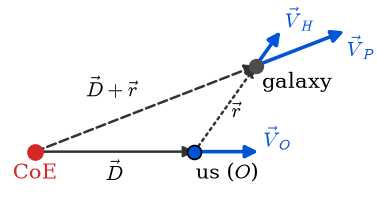
\includegraphics[width=0.48\textwidth]{L01a_geometry_top.png}\hfill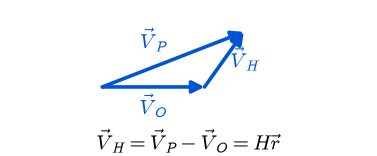
\includegraphics[width=0.48\textwidth]{L01a_geometry_bot.png}\caption{\textbf{[unchanged from rev6: schematic from the original preprint; generating script not located]}\ Hubble velocity vectors for the CoE, the observer and a galaxy, $\vec V_H=\vec V_g-\vec V_O$ (rev6 Fig.~1 top and middle). Labels predate rev7; the rev7 numbers are in Fig.~\ref{fig:setup}.}\label{fig:setup0}\end{figure} is the candidate.
\subsection{Cluster observables in detail (rev6 text)}
For an isotropic universe both ratios would be 1 in every direction. What the data show is the residual from 1, and that residual, not a fitted curve, is what the CoE model must reproduce.

Migkas et al.\ test sky isotropy with the X-ray luminosity--temperature relation of galaxy clusters. $L_X$ depends on luminosity distance and $T$ does not, so a directional change in the normalisation $A$ traces a directional distance or expansion scale. With $A\,H_0^2$ held fixed, $H/H_{\rm ref}=1/\sqrt{A/A_{\rm all}}$, so troughs in $A/A_{\rm all}$ are directions of higher apparent expansion rate, provided the variation is cosmological rather than a cluster or X-ray systematic. The slope $B$ is set more by sample composition. Both are given in sliding cones of width $\Delta l=90^\circ$ against Galactic longitude (their Fig.~6), digitised here at 71 points (Fig.~\ref{r6:fig:obsAB}).

Two features matter for what follows. $A/A_{\rm all}$ has two humps and two troughs over $360^\circ$, with its deepest low near $l\approx255$--$270^\circ$; $B/B_{\rm all}$ varies more slowly, with one broad low and one broad high. The curves in Fig.~\ref{r6:fig:obsAB} are the author's spreadsheet model with a one-cycle phase rotation, $(1\mp{\rm Amp}\,\sin(l+\varphi))$ times the shell series, Amp $=\mp0.06$, $\varphi=0.35$\,rad; it is a diagnostic phase alignment, not a free dipole fit. Against the spreadsheet series the rotation raises $R^2$ for A from 0.501 to 0.739 and for B from 0.372 to 0.733; against the digitised points, from 0.446 to 0.712 (A) and from 0.483 to 0.785 (B). Source: \texttt{migkas\_bars\_rotation\_summary.json}.

\begin{figure*}[t]\centering\fig{0.68\textwidth}{0.6\textheight}{R04_migkas_rotation.png}\caption{\textbf{[REGEN rev7: original script re-run (\texttt{fig7/rerun/L04\_migkas\_rotation.py}); data figure, independent of the LTB background]}\ The observables. Top: Migkas $A/A_{\rm all}$ against Galactic longitude (digitised, $\Delta l=90^\circ$ cones, black with error bars). Bottom: $B/B_{\rm all}$. Solid: spreadsheet shell model with the one-cycle sine rotation (Amp $=\mp0.06$, $\varphi=0.35$\,rad); dashed: best shared-$\varphi$ scan. $R^2$ before and after rotation is given in each panel. Restored from \texttt{cosmology/figures}.}\label{r6:fig:obsAB}\end{figure*}
\subsection{rev6 supporting text}
This section keeps the rev6 text for the analyses that rev7 did not redo, so nothing is silently dropped. The text was written on the earlier background ($D=42$\,Gpc for the web, a source shell at $R\approx4$\,Gpc for the stochastic field), which rev7 replaces with the single LTB background of \S\ref{sec:bg} ($D=34.96$\,Gpc, $R=0.18957$\,Gpc); numbers in the running text belong to that stage unless stated. Every figure in this section has been regenerated from a script for rev7 and is tagged \REGEN, with its caption carrying the rev7 numbers. Where a rev6 analysis has no meaning on the new background (the $R=4/8/14$\,Gpc domain scan, the stage-A $\lambda$ L-curve), the caption says why and shows the rev7 counterpart. Appendix~B lists every figure with its script.
\subsection{Rings, the Migkas overlay and rotation}\label{r6:sec:rings}
The fit above matches $A$ along longitude only. The residual it leaves is in the morphology on the full sky: where the maxima, minima and rings fall. That is tested here, with the geometry held fixed.

\paragraph{Rings.} Off-centre placement gives closed curves of constant phase $\varphi(\psi)$ on the sky: rings about the CoE axis. In the original preprint the low-redshift ring and the longitude dependence of $A/A_{\rm all}$ were fixed from the geometry before the comparison with the Migkas maps (its Fix Point~1); the Migkas data were not used to add a morphological degree of freedom.

\begin{figure*}[t]\centering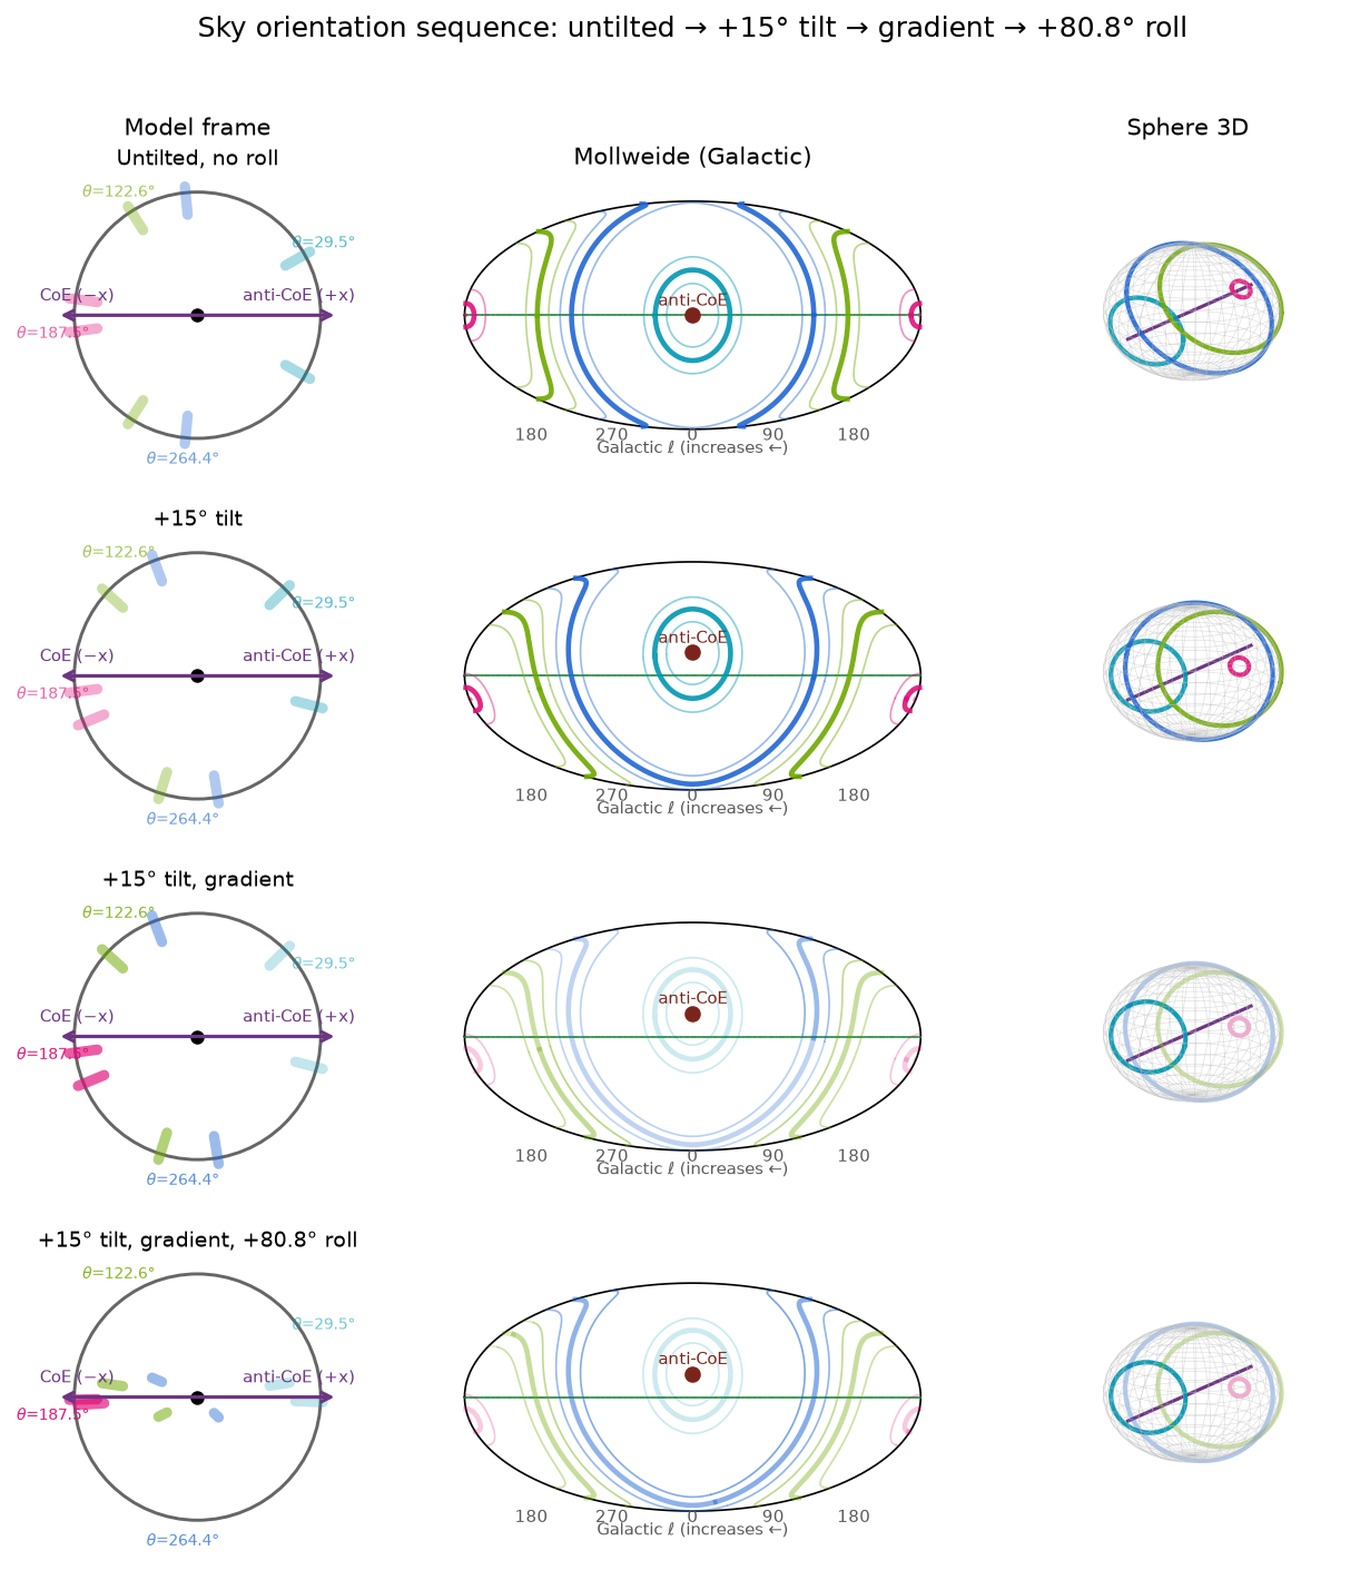
\includegraphics[width=\textwidth]{R08_sky_orientation.jpg}\caption{\textbf{[REGEN rev7: original maker re-run (\texttt{fig7/rerun/L08\_sky\_orientation.py}); orientation construction, independent of the LTB background]}\ Sky-orientation sequence: untilted configuration, then $+15^\circ$ tilt, radial gradient, and $+80.8^\circ$ roll about the CoE axis. Restored from the original preprint (its Fig.~5).}\label{r6:fig:orient}\end{figure*}

\paragraph{Tilt, gradient and roll.} The full longitude profile, with the band positions and the residual bars they leave, is shown in Fig.~[rev6]. The model is placed on the sky in three steps, starting from an untilted configuration with no roll: a $+15^\circ$ tilt of the CoE axis (anti-CoE near $(l,b)=(0^\circ,+15^\circ)$), a radial gradient, and a $+80.8^\circ$ roll (yaw) about the CoE axis (Fig.~\ref{r6:fig:orient}). Fig.~\ref{r6:fig:overlay} overlays the resulting maximum and minimum bands on Migkas Fig.~8. Each band is $18^\circ$ end to end ($\pm9^\circ$, 5\% of $360^\circ$). The Migkas maxima include $(17^\circ,-9^\circ)$ and $(185^\circ,0^\circ)$. The residual maps in \S\ref{r6:sec:skyres} use a later orientation of the same kind, a $15^\circ$ lift and a $45^\circ$ counterclockwise rotation; the two orientations are reported as they were made and have not been reconciled.

\paragraph{How much the rotation adds.} In the original preprint's fits to $A/A_{\rm all}$ (null $\chi^2=45.14$), a point mass at the CoE without rotation gives $R^2=0.521$; with rotation and the one-cycle phase factor $R^2$ rises to 0.845 (exponential law, CatWISE lock) and 0.870 (soft core). These are unweighted $R^2$ values from that draft and are not recomputed here. The amplitude is partly set by how the construction is normalised (the density--distance trade); the morphology is the part that was not tuned.

\begin{figure*}[p]\centering\fig{\textwidth}{0.9\textheight}{R09_overlay_bands.png}\caption{\textbf{[REGEN rev7: \texttt{R09\_overlay\_bands.py} runs the original band code; band centres checked against the rev7 $D=34.96$ refit, whose extrema ($l=20^\circ,200^\circ$ max; $127^\circ,272^\circ$ min) equal the locked curve's]}\ Predicted MAX/MIN bands on Migkas Fig.~8 (two MAX and two MIN bands, each $18^\circ$ wide) for the $+15^\circ$ tilt alone (top), tilt with gradient (middle), and tilt, gradient and $+80.8^\circ$ roll (bottom).}\label{r6:fig:overlay}\end{figure*}

\subsection{The CMB: what keeps the sky flat}\label{r6:sec:flatcmb}
If the off-centre geometry is real, the anisotropy it puts into $A$ and $B$ should also appear on the last-scattering surface. The observed CMB is isotropic to $\sim10^{-5}$ after the dipole. That near-absence is the residual the rest of these notes work on.

Holding the geometry fixed and carrying it to last scattering ($z_\star\approx1100$), the original preprint found a geometric multipole of several percent on the CMB sky, orders of magnitude above the Planck isotropy level. Geometry alone is therefore incomplete. That draft then added special-relativistic Doppler and central-mass gravitational redshift, which together cancelled 95.9\% of the geometric RMS while keeping the low-$z$ morphology (its Fix Point~2). The model must therefore say what distribution of matter around the off-centre observer gives a nearly flat CMB sky and, at the same time, the Planck $TT$ spectrum. The following subsections use the tools of \S\ref{sec:methods} (harmonics, cosmic variance, $\chi^2$) and build a realistic void/cluster web, the stochastic field and its projection, and then fit the spectrum as a fixed background plus acoustic and damped terms. The residuals that remain are taken back to the $A$/$B$ sky in \S\ref{r6:sec:skyres}.

\subsection{Matching target spectra}


\paragraph{Primers.} An axisymmetric pattern ($m=0$) is a sum of Legendre polynomials $P_\ell(\cos\theta)$, so a single $P_\ell$ puts all its power in one $\ell$ (Fig.~\ref{r6:fig:h1}). $N$ equal masses equally spaced on a ring have azimuthal Fourier power only at multiples of $N$ (aliasing). Binary mixtures and quadrature masses behave the same way. \emph{Matching a target}: given a target $C_\ell$, find over-/under-densities that produce it. Because $C_\ell$ discards the phases of the $a_{\ell m}$, the solution is degenerate (Figs.~\ref{r6:fig:h1}--\ref{r6:fig:inv}).
\paragraph{Web and kernel ladder.} Before targets were matched, hand-placed masses were replaced by a statistically realistic web of clusters and voids (Fig.~\ref{r6:fig:web}), and its sky imprint was evaluated on spheres of radius $R$ around the observer, the kernel ladder of Fig.~\ref{r6:fig:ladder}. How the web is built and how the ladder is read are given in \S\ref{r6:sec:web}.


\subsection{A realistic web of voids and clusters}\label{r6:sec:web}
Hand-placed masses are a model whose residuals depend on the hand. A statistical web replaces them so that whatever structure remains in the projected field is not an artefact of where objects were put.

\paragraph{Purpose.} Hand-placed masses are replaced by a statistically realistic population. Each body sources a Newtonian potential, and the sky signal is the gravitational field sampled on spheres around the observer.

\paragraph{Ingredients (from \texttt{realweb/build.py}, \texttt{cosmo.py}).} Background: $h=0.7$, $\Omega_m=0.31$, $\Omega_b=0.049$, $n_s=0.965$, $\sigma_8=0.8$, $\bar\rho_m=\Omega_m\,2.775\times10^{11}h^2=4.215\times10^{10}\,M_\odot$Mpc$^{-3}$. Linear spectrum $P(k)=Ak^{n_s}T_{\rm EH}^2(k)$ (Eisenstein--Hu no-wiggle transfer function). $A$ is fixed by $\sigma^2(R)=\int\frac{k^2dk}{2\pi^2}P(k)W^2(kR)=0.8^2$ at $R=8/h$\,Mpc, with the top-hat $W(x)=3(\sin x-x\cos x)/x^3$.

\FIGc{R15_web_ingredients.png}{0.26}{\textbf{[REGEN rev7: \texttt{R15\_web\_ingredients.py} computes from \texttt{cosmo.py}; standard-cosmology inputs, independent of the CoE background]}\ Web ingredients: Press--Schechter halo mass function with the Eisenstein--Hu $P(k)$ (left), Sheth--van de Weygaert void size function (middle), compensated void with its ridge holding the missing mass (right; enclosed excess returns to 0 at $1.5R_v$).}{r6:fig:webd}
\emph{Clusters}, Press--Schechter. A region of mass $M=\tfrac43\pi R^3\bar\rho_m$ collapses when its linear overdensity exceeds $\delta_c=1.686$. The fraction above threshold is ${\rm erfc}(\nu/\sqrt2)$ with $\nu=\delta_c/\sigma(M)$; differentiating with respect to $\ln M$ and multiplying by $\bar\rho_m/M$ gives
\begin{equation}\label{r6:eq11}
\frac{dn}{d\ln M}=\sqrt{\tfrac2\pi}\frac{\bar\rho_m}{M}\nu\Big|\frac{d\ln\sigma}{d\ln M}\Big|e^{-\nu^2/2},
\end{equation}
for $M=10^{14}$--$2\times10^{15}M_\odot$ (41 bins). The peak-background bias is $b=1+(\nu^2-1)/\delta_c$: halos are more numerous where the large-scale $\delta_{\rm lin}>0$.

\emph{Voids}, Sheth--van de Weygaert (2004). This is the two-barrier excursion-set size function with void threshold $\delta_v=-2.7$, evaluated at linear radius $R_L=R/1.7$ for $R=10$--50\,Mpc. Bias $-1.5$. A void of radius $R_v$ has interior contrast $-0.85$, i.e.\ mass deficit $M_d=0.85\bar\rho_m\tfrac{4\pi}{3}R_v^3$. Example: $R_v=30$\,Mpc gives $M_d=4.0\times10^{15}M_\odot$. It is painted as $-M_d$ at the centre plus 8 random points of $+M_d/8$ on a shell at $1.25R_v$, so each void is compensated (net mass zero).

\emph{Placement.} Counts per cell are Poisson with mean
\begin{equation}\label{r6:eq12}
\lambda=\frac{dn}{d\ln X}\Delta\ln X\,\Delta V\,\max(0,1+b\,\delta_{\rm lin})\,m(\mathbf x)\,f ,
\end{equation}
with $X=M$ or $R_v$, thinning $f=1/100$, and $m(\mathbf x)$ the CoE modulation of Fig.~\ref{r6:fig:mod}. The painted $\rho$ is mean-subtracted inside the region (zero net mass), then $\Phi$ is found by FFT Poisson (\S\ref{r6:sec:field}).

\paragraph{The kernel ladder: what ``kernel at $R$'' means.} From \texttt{realweb/build.py} (\texttt{skyfrom}) and \texttt{mc/mc.py}, \texttt{mc\_samples.py}. \emph{Step 1, acceleration}: $\mathbf a=-\nabla\Phi$ on the grid, from Poisson in Fourier space, $\mathbf a_k=-i\mathbf k\,(4\pi G\rho_k/k^2)$, with a Gaussian of cell width applied to represent finite body size. \emph{Step 2, radial tidal signal on a sphere}: for each HEALPix direction $\hat n$ ($N_{\rm side}=32$, 12{,}288 directions) and each radius $R\in\{0.5,0.9,2,4,8,14\}$\,Gpc,
\begin{equation}\label{r6:eq13}
s_R(\hat n)=\big[\mathbf a(R\hat n)-\mathbf a(\mathbf 0)\big]\cdot\hat n-\langle\cdot\rangle_{\rm sky}.
\end{equation}
This is the radial component of the acceleration at distance $R$ \emph{relative to the observer's own acceleration}: a tidal (differential) field, since a uniform acceleration is unobservable. ``Kernel at $R$ Gpc'' therefore means that the web's sky imprint is evaluated on the sphere of radius $R$. Small $R$ weights nearby structure; large $R$ samples the field near the source surface. The map is multiplied by $M_\odot/K_G\cdot R_V^2$ ($K_G=7.7\times10^{51}/0.0039$, $R_V=14.3$) to put it in the same dimensionless units as the deterministic ``red'' map. \flag{the physical origin of the constant $K_G$}. \emph{Step 3, Monte-Carlo universe}: each universe has a new Gaussian $\delta_{\rm lin}$ and Poisson halos in 8 mass bins (voids omitted in the fast variant, $N=256$ grids, seeds $500000+i$). \emph{Step 4, the \% levels}: the sky analysed is


\noindent\emph{Reading Fig.~\ref{r6:fig:ladder}.} Coloured curves: $D_\ell$ of $\Theta_{\rm red}+\epsilon s_R$ for the listed $\epsilon$; magenta: best $\epsilon$; red dashed: smooth red alone; black line: ΛCDM ($\chi^2=20.1$); points: Planck. The title colours and ``my guess'' labels come from the plotting script.
\begin{equation}\label{r6:eq14}
\Theta_\epsilon(\hat n)=\Theta_{\rm red}(\hat n)+\epsilon\,s_R(\hat n),
\end{equation}
with $\Theta_{\rm red}$ the smooth axisymmetric CoE background (\texttt{sm\_red}, $\Theta_{\rm red}=e^{-S(\psi)}/\langle e^{-S}\rangle-1$, with $S$ a spline in angle $\psi$ from the axis). For each $\epsilon\in\{100,50,20,10,5,2,1,0.5,0.2,0.05\}\%$ the code computes $D_\ell$ via Eq.~([rev6]) and $\chi^2$ via Eq.~([rev6]). So ``10\%'' means the web field is scaled to one tenth of its natural (strength-1) amplitude before being added to the background; since $D_\ell$ is quadratic in the map, its web part scales as $\epsilon^2$. The ``best'' curve minimises $\chi^2$ over 60 log-spaced $\epsilon$ from $10^{-3.5}$ to $10^{0.3}$ (0.03\%--200\%). \emph{Reading the ladder}: as $\epsilon\to0$ the curves converge on the smooth-red spectrum (dashed red, $\chi^2=471.4$ in the figure legends), whose power sits in odd $\ell$ because it is axisymmetric. Increasing $\epsilon$ fills in the even $\ell$ and raises the overall level.

\paragraph{Labels on Fig.~\ref{r6:fig:ladder}.} The panel titles carry ``my guess: PASS/FAIL'' labels written by \texttt{mc\_samples.py}. Its rule is: PASS if $\chi^2_{\rm best}\le100$, $|$slope of $\ln D_\ell$ vs $\ell$ over $\ell$ 4--30$|<0.05$, and $\max D_{2..4}/\max D^{\rm Planck}_{2..4}<2.5$. These are the script's labels, reproduced in the figure; no verdict is drawn here. Recorded values for universe \#3 (\texttt{samples/guesses.json}), as $R$: $\epsilon_{\rm best}$, $\chi^2$: 0.5: 29.0\%, 441.6; 0.9: 25.0\%, 411.5; 2: 25.0\%, 177.2; 4: 21.6\%, 69.6; 8: 52.5\%, 85.0; 14: 45.3\%, 47.2. \flag{at 8\,Gpc the JSON records the low-$\ell$ ratio 2.99, which exceeds the coded 2.5 threshold, yet the label is PASS: the JSON and the script as now written disagree}.

\subsection{Stochastic field and sky projection}\label{r6:sec:field}
A random field predicts only an ensemble mean $C_\ell$, so the residual between one realisation and the mean is expected and is bounded by cosmic variance; only residuals beyond that band are informative.

\paragraph{Why a random field.} Instead of placing objects, the density contrast $\delta(\mathbf x)=\rho/\bar\rho-1$ is treated as a zero-mean Gaussian random field. In Fourier space $\langle\delta_{\mathbf k}\delta^*_{\mathbf k'}\rangle=(2\pi)^3\delta^3(\mathbf k-\mathbf k')P_\delta(k)$, where $P_\delta$ [Gpc$^3$] is the variance per mode. The model predicts the \emph{ensemble mean} $C_\ell$; one sky scatters about it by Eq.~([rev6]).

\paragraph{Poisson equation.} Newtonian gravity: $\nabla^2\Phi=4\pi G\bar\rho\,\delta$. Fourier transforming ($\nabla\to i\mathbf k$, so $\nabla^2\to-k^2$),
\begin{equation}\label{r6:eq15}
\Phi_{\mathbf k}=-\frac{4\pi G\bar\rho}{k^2}\delta_{\mathbf k}\ \Rightarrow\ P_\Phi=\frac{(4\pi G\bar\rho)^2}{k^4}P_\delta .
\end{equation}
Code units: $G=4.30\times10^{-12}$\,Gpc(km/s)$^2M_\odot^{-1}$ and $\bar\rho=4.215\times10^{19}M_\odot$Gpc$^{-3}$, so $4\pi G\bar\rho=2.278\times10^9$\,(km/s)$^2$Gpc$^{-2}$. Example: a mode with $k=1$\,Gpc$^{-1}$ and $\delta_k=10^{-4}$ gives $|\Phi|=2.28\times10^5$\,(km/s)$^2$, i.e.\ $\Phi/c^2=2.5\times10^{-6}$. Meaning: the $k^{-2}$ makes the potential dominated by large scales.
\why{Valid for $|\Phi|/c^2\ll1$, non-relativistic sources, and scales well inside the horizon ($kR\gg1$). At $\ell\lesssim3$, where $k\sim1/R$, relativistic (GR) corrections are not negligible. The code also evaluates the moving lens with the full CoE radial velocity, which is superluminal ($\dot R\approx4c$ today per the stage-A notes); the Newtonian treatment of that regime is a model assumption, not a derived result.}

\paragraph{Source terms and the moving lens.} A photon crossing a potential picks up (i) Sachs--Wolfe $\Theta=\Phi/3c^2$ at the source, (ii) integrated Sachs--Wolfe $\frac{2}{c^2}\int\dot\Phi\,dt$ if $\Phi$ evolves, and (iii) the moving-lens term. If the lens moves with transverse velocity $\mathbf u$, the potential the photon sees changes during the crossing, giving $\Theta\propto\frac{2}{c^2}\int d\chi\,(\text{time per }d\chi)\,\mathbf u\cdot\nabla\Phi$. In \texttt{fwd.py} this is the kernel $K_M(\chi)=\frac{2}{c^2}\big[-\frac{\bar A}{a}\frac{\Delta t}{\Delta\chi}\,42\,R_d\big]$ multiplying $\mathbf u\cdot\nabla\Phi_0$ [(km/s)$^2$/Gpc]. Here $\bar A$ is the growth factor $D/a$, $\Delta t/\Delta\chi$ the time spent per unit path, $42\,R_d$ the CoE radial-velocity factor tabulated from \texttt{flowR.py}, and $\chi$ the distance from the observer. The stage-A README reports that the moving lens is $\ge99.99\%$ of the field's power (SW+ISW $\le9\times10^{-5}$), so only $K_M$ is kept in the Limber part. \flag{the closed form of $R_d$; it is taken from tabulated \texttt{tab.npz}}.

\emph{The $k^2/3$ factor.} $\mathbf u\cdot\nabla\Phi\to i(\mathbf k\cdot\mathbf u)\Phi_{\mathbf k}$. Averaging over random orientations of $\hat k$ relative to $\mathbf u$: $\langle(\hat k\cdot\hat u)^2\rangle=\frac{1}{4\pi}\int\cos^2\theta\,d\Omega=\tfrac13$, so the power is multiplied by $u^2k^2/3$, with $u$ absorbed into $K_M$.

\paragraph{Radial window.} The field is confined to a shell, $\Phi(\chi\hat n)=W(\chi)\phi_g$, with
\begin{equation}\label{r6:eq16}
W(\chi)=\exp\!\Big[-\frac{(\chi-R_c)^2}{2w^2}\Big],
\end{equation}
centre $R_c$ and width $w$ [Gpc]. \emph{Why Gaussian}: two parameters, smooth (no edge artefacts in $\ell$), and its derivative $W'=-W(\chi-R_c)/w^2$ is analytic. That derivative is needed because $\mathbf u\cdot\nabla(W\phi)=W\,\mathbf u\cdot\nabla\phi+\phi\,W'(\hat n\cdot\mathbf u)$. Fitted: $R_c=3.5715$, $w=0.3355$\,Gpc with $R=4$. The source surface at 4\,Gpc is $(4-3.5715)/0.3355=1.28w$ above the centre, so the path truncates the Gaussian. That truncation is why Limber needs correcting (below).
\why{A Gaussian is a parametrisation, not a derived shell profile. It fails to represent sharp-edged or multi-shell structures.}

\paragraph{Exact projection (derivation).} \emph{Step 1}: the line-of-sight integral is $\Theta(\hat n)=\int d\chi\,K(\chi)W(\chi)\,\Phi(\chi\hat n)$. \emph{Step 2}: Fourier expand, $\Phi(\chi\hat n)=\int\frac{d^3k}{(2\pi)^3}\Phi_{\mathbf k}e^{i\mathbf k\cdot\hat n\chi}$, and use the plane-wave expansion $e^{i\mathbf k\cdot\hat n\chi}=4\pi\sum_{\ell m}i^\ell j_\ell(k\chi)Y_{\ell m}(\hat n)Y^*_{\ell m}(\hat k)$. \emph{Step 3}: read off $a_{\ell m}=\frac{i^\ell}{2\pi^2}\int d^3k\,\Phi_{\mathbf k}Y^*_{\ell m}(\hat k)\Delta_\ell(k)$ with $\Delta_\ell(k)=\int d\chi\,KWj_\ell(k\chi)$. \emph{Step 4}: take $\langle|a_{\ell m}|^2\rangle$ with the power-spectrum definition. The $\delta^3$ collapses one $k$ integral and $\int d\Omega_k|Y_{\ell m}|^2=1$, giving
\begin{equation}\label{r6:eq17}
C_\ell=\frac{2}{\pi}\int k^2dk\,P_\Phi(k)\,|\Delta_\ell(k)|^2 .
\end{equation}
$j_\ell$ is the spherical Bessel function: the radial profile of a plane wave's $\ell$-th multipole. For the moving lens, $P_\Phi\to\frac{k^2}{3}P_\Phi$, and \texttt{fwd.py} evaluates the $W'$ term exactly with $\cos\theta$ Gaunt couplings to $\ell\pm1$. This is used for $\ell\le50$.

\paragraph{Limber approximation (derivation).} For large $\ell$, $j_\ell(k\chi)$ is sharply peaked at $k\chi\approx\nu\equiv\ell+\tfrac12$. Using the closure relation $\int k^2dk\,j_\ell(k\chi)j_\ell(k\chi')=\frac{\pi}{2\chi^2}\delta(\chi-\chi')$, and assuming $P_\Phi$ varies slowly over the width of $j_\ell$ so it can be evaluated at $k=\nu/\chi$, Eq.~(\ref{r6:eq17}) collapses to a single integral:
\begin{equation}\label{r6:eq18}\begin{split}
D_\ell\simeq&\frac{\ell(\ell+1)T_0^2}{2\pi}\int d\chi\\
&\times\frac{[K_MW]^2}{\chi^2}\frac{k^2}{3}P_\Phi(k)\Big|_{k=\nu/\chi}.
\end{split}\end{equation}
Meaning: each multipole receives power only from the wavenumber that projects to angle $1/\ell$ at distance $\chi$. Only transverse modes contribute; radial modes cancel along the line of sight.
\why{It requires the kernel $K_MW$ to vary slowly compared with $j_\ell$'s oscillation $\sim\chi/\nu$, i.e.\ $\ell\gg R_c/w=3.5715/0.3355=10.6$, and no sharp edges. Checks in \texttt{acoustic\_limber\_check*.json}: interior or broad shells agree within 3\% for $\ell\ge150$, and a 0.5\,Gpc shell within 0.3\% even at $\ell=20$. Shells cut off at the path end (as here) are overestimated by about $1.5$--$5\times$ below $\ell=150$ and by up to $\pm20\%$ near $\ell=300$.}

\paragraph{Exact/Limber correction.} Hence $D^{\rm used}_\ell=c_\ell D^{\rm Limber}_\ell$ for $\ell>50$, with $c_\ell=C^{\rm exact}_\ell/C^{\rm Limber}_\ell$ computed by Eq.~(\ref{r6:eq17}) at 69 nodes. The nodes are $\ell=50,55,60,70,80,90,100,115,130,150,175$, then 200 to 2480 in steps of 40. $c_\ell$ is interpolated in $\ln\ell$ and recomputed after each fit pass, because it depends on $R_c$ and $w$.

\paragraph{Fitted source spectrum.} 
\begin{equation}\label{r6:eq19}\begin{split}
P_\delta=&10^{\lg A}k^{n}e^{-(k/k_D)^2}\big[1+A_w\cos(kr_s+\phi)\\
&+Be^{-k/k_B}\cos(kr_2+\phi_2)\big],
\end{split}\end{equation}
with $k$ in Gpc$^{-1}$ and $P_\delta$ in Gpc$^3$. Term by term: $k^n$ is the broadband tilt; $e^{-(k/k_D)^2}$ is a small-scale damping cutoff; $A_w\cos(kr_s+\phi)$ is an oscillation in $k$ with period $2\pi/r_s$, i.e.\ a preferred comoving separation $r_s$ (acoustic-like); the $B$ term is a second, decaying oscillation. Fitted ($r_2$ free, \texttt{acoustic\_half\_fixed.json}): $\lg A=-8.282$, $n=-0.183$, $A_w=0.311$, $r_s=79.5$\,Mpc, $\phi=1.367$, $k_D=335$\,Gpc$^{-1}$, $B=0.815$, $k_B=138$\,Gpc$^{-1}$, $r_2=42.1$\,Mpc, $\phi_2=3.640$. Example: at $k=100$\,Gpc$^{-1}$, $10^{-8.282}\times100^{-0.183}\times e^{-0.089}=2.2\times10^{-9}$\,Gpc$^3$ before the bracket.

\paragraph{Mapping $\Delta\ell\leftrightarrow r$ via $\ell\approx k\chi$.} From Limber, a wavenumber $k$ at distance $\chi$ appears at $\ell\approx k\chi$. An oscillation $\cos(kr_s)$ has period $\Delta k=2\pi/r_s$, so on the sky its peaks are spaced by
\begin{equation}\label{r6:eq20}
\Delta\ell\approx\chi_{\rm eff}\Delta k=2\pi\chi_{\rm eff}/r_s .
\end{equation}
Example: acoustic fit, $R_c=3.944$\,Gpc, $r_s=0.0819$\,Gpc, gives $\Delta\ell=302.6$; the model peaks 227, 530, 831, 1131, 1431 are spaced 300--303. For the final fit, $R_c=3.5715$ and $r_s=0.0795$ give 282, whereas the model peaks are spaced $\approx300$. That implies $\chi_{\rm eff}=300\times0.0795/2\pi\approx3.8$\,Gpc, larger than $R_c$ because $K_M$ rises toward the source and the truncated window is skewed. Conversely, an angular feature at $\ell$ has physical size $\chi\theta$ with $\theta=\pi/\ell$. For $\ell=220$: 57.1, 114.2, 199.9\,Mpc at $\chi=4$, 8, 14\,Gpc.
\why{It holds where Limber holds and for thin kernels. It fails at low $\ell$ and for broad kernels, where many $\chi$ contribute and $\chi_{\rm eff}$ is ambiguous.}

\subsection{The fixed low-$\ell$ background $D^{\rm fix}_\ell$}
The deterministic, axisymmetric part of the CoE sky is modelled out once as $D^{\rm fix}_\ell$, so that the later fits work on the residual above this background.

\paragraph{Definition (from \texttt{fit.py}).} The CoE sky has a deterministic, axisymmetric part: the smooth red map plus an \texttt{rs\_cc} map. Its spectrum is computed once,
\begin{equation}\label{r6:eq21}
D^{\rm fix}_\ell=\frac{\ell(\ell+1)}{2\pi}T_0^2\,\hat C_\ell\big[\Theta_{\rm red}+\Theta_{\rm rs\_cc}\big],\quad 2\le\ell\le30,
\end{equation}
with the dipole removed, and stored in \texttt{fit\_l30\_bg.json}. It is added to the field: $D^{\rm model}_\ell=c_\ell D^{\rm field}_\ell+D^{\rm fix}_\ell$. \emph{Why add powers}: the field has zero mean and is independent of the background, so $\langle|a^{\rm bg}+a^{\rm f}|^2\rangle=|a^{\rm bg}|^2+\langle|a^{\rm f}|^2\rangle$ (the cross term averages to zero). \emph{Values}: $\ell=3$: 1506.4\,$\mu$K$^2$; $\ell=2$: 0.1; all others $\le5.1$, with odd $\ell$ (5, 7, \ldots) carrying 0.3--5.1 and even $\ell\ge4$ essentially 0. The odd/even pattern is the axisymmetric signature: an odd-parity profile about the axis projects onto odd Legendre polynomials. It is held fixed (no free parameters) and has no cosmic-variance band, since it is deterministic. Above $\ell=30$ it is set to zero; its power is already negligible above $\ell=3$. \flag{the physical definition of \texttt{rs\_cc}}.

\subsection{Acoustic fit and residual decomposition}
After the fixed background, an acoustic stochastic term is fitted. Its residual against Planck is still large (the $\chi^2$ and $r^2$ below are worse than ΛCDM), and the oscillatory structure left in that residual is what the damped model of the next section is built to describe.

\paragraph{Acoustic fit.} Eq.~(\ref{r6:eq19}) without the $B$ term, eight free parameters with $R_c$ and $w$ free (``free\_W''). Result: $r_s=81.9$\,Mpc, $R_c=3.944$\,Gpc; $\chi^2_{2-2500}=11{,}772$, Pearson $r^2=0.871$ (ΛCDM: 2{,}558, 0.983). Peaks: CoE 227, 530, 831, 1131, 1431 vs Planck 224, 535, 821, 1122, 1412.

\paragraph{Residuals.} Normalised residual: $\epsilon_\ell=(D^{\rm P}_\ell-D^{\rm CoE}_\ell)/\sigma_\ell$, dimensionless (in $\sigma$). Two linear models with $s_j(\ell)=\sin(2\pi j\ell/\Delta\ell+\phi_j)$:
\begin{align}
\text{undamped: }&\epsilon_\ell=\textstyle\sum_ja_js_j(\ell),\label{r6:eq22}\\
\text{damped: }&\epsilon_\ell=e^{-\ell/L}\textstyle\sum_ja_js_j(\ell).\label{r6:eq23}
\end{align}
\emph{Why harmonics}: if the model's peak spacing or shape is slightly off, the residual is periodic in $\ell$ with the spacing error. $j=2$ is the half period, which is the signature of an odd/even peak alternation. \emph{Why damping}: $\sigma_\ell$ shrinks and the signal falls with $\ell$, so the misfit in $\sigma$ units decays. A single envelope $e^{-\ell/L}$ adds one parameter. \emph{Fit}: for fixed $(\Delta\ell,L)$ the model is linear in $a_j\cos\phi_j$, $a_j\sin\phi_j$ (least squares), and $\Delta\ell$, $L$ are scanned. Results: undamped plateaus at $r^2=0.551$; damped, 1--9 harmonics give $r^2=$ 0.797, 0.813, 0.831, 0.834, 0.835, 0.836, 0.836, 0.837, 0.837, with $\Delta\ell\approx593$ and $L\approx990$. Starting amplitudes ($\sigma$): 34.6, 5.6, 5.7, 2.2, 1.3, 1.0, 1.2, 0.4, 0.5. \flag{these values were taken from the earlier figure set; the script was not re-run}. The decomposition is purely descriptive. It fails where the residual structure is not stationary, e.g.\ the late troughs at $\ell\sim1400$, 2000, which the shared envelope has already suppressed.

\paragraph{Mapping to source parameters.} Using Eq.~(\ref{r6:eq20}) with $\chi\approx3.94$\,Gpc: a residual period $\Delta\ell=593$ corresponds to $r_2=2\pi\times3.94/593=0.0417$\,Gpc $=41.7$\,Mpc$\,\approx r_s/2$. An envelope $e^{-\ell/L}$ with $\ell=k\chi$ becomes $e^{-k\chi/L}$, so $k_B=L/\chi=990/3.94=251$\,Gpc$^{-1}=0.25$\,Mpc$^{-1}$. These were the starting values for the damped term.

\par\medskip\noindent\begin{minipage}{\columnwidth}\centering\footnotesize\setlength{\tabcolsep}{4pt}
\captionof{table}{Fit statistics (Planck errors). Pearson $r^2$ over $\ell$ 2--2500.}\label{r6:tab:fit}
\begin{tabular}{lccc}\toprule
Model & $\chi^2_{2-2500}$ & $r^2$ & $\chi^2_{2-30}$\\\midrule
CoE $r_2$ free & 3{,}787 & 0.976 & 137\\
CoE half ($r_2=r_s/2$) & 4{,}131 & 0.966 & 49.1\\
CoE acoustic (no $B$) & 11{,}772 & 0.871 & --\\
ΛCDM & 2{,}558 & 0.983 & 20.1\\\bottomrule
\end{tabular}\\[6pt]
\begin{tabular}{cccc}\toprule
peak & Planck & CoE $r_2$ free & CoE half\\\midrule
1&228 (5726)&218 (5927)&207 (5223)\\
2&544 (2580)&531 (2449)&537 (2383)\\
3&823 (2525)&813 (2466)&818 (2433)\\
4&1121 (1239)&1130 (1293)&1132 (1260)\\
5&1417 (814)&1420 (822)&1426 (861)\\\bottomrule
\end{tabular}\\[2pt]
Lower: peak $\ell$ ($D_\ell$ in $\mu$K$^2$).
\end{minipage}\par\medskip
\subsection{Damped half-scale model}
The second damped mode is a hypothesis taken from the acoustic-fit residual. Here it is added to the model and refitted, and the question is how much of that residual structure it removes.
\noindent\textit{rev6 Fig.~24 (this model at $R=4$\,Gpc, $\chi^2_{2-2500}=3{,}787$) is replaced by its rev7 regeneration, Fig.~\ref{fig:tt}.}

\paragraph{Model and fit.} Eq.~(\ref{r6:eq19}) with all 12 parameters $(\lg A,n,A_w,r_s,\phi,k_D,R_c,w,B,k_B,r_2,\phi_2)$ floated in one $\chi^2$ minimisation over $\ell=2$--2500 (Eq.~([rev6])). The ``half'' variant ties $r_2=r_s/2$ (11 parameters). Result ($r_2$ free): $r_2=42.1$\,Mpc vs $r_s/2=39.8$; $k_B=0.138$\,Mpc$^{-1}$, against the starting 0.25. The resulting model is shown in Fig.~[rev6].

\paragraph{The $\ell=50$ step.} A ratio $c_\ell$ computed for an earlier, narrower shell had been left in place when the fit widened the shell, which produced a step at $\ell=50$ (reported as 43\%). Recomputing $c_\ell$ on the 69 nodes at each pass reduces the 50$\to$51 change to $\approx1.1\%$. \flag{the 43\% and 1.1\% figures come from the run log; not re-measured here}.
\paragraph{Remaining structure.} The odd/even alternation is absent from the new residual. What remains: a slow wave with $\Delta\ell\approx1{,}384$ ($\pm8$--$11\sigma$), and $\ell=2$--3 raised to $\approx3{,}300\,\mu$K$^2$, which dominates $\chi^2_{2-30}=137$; part of the $\ell=3$ level is $D^{\rm fix}_3=1506$. \flag{the $\Delta\ell\approx1384$ amplitude and the 3300\,$\mu$K$^2$ level were read from the earlier figures}.

\subsection{Residual harmonics against independent sky anomalies}\label{r6:sec:skyres}
The A and B residuals left by the CoE model are peeled layer by layer, $F_1+F_2+F_3$ for $n=1$, 2, 3, each fitted to what the previous layer left. The leftover map is then compared with sky anomalies found independently. Agreement there is qualitative and is reported as such.

\begin{figure*}[t]\centering\fig{\textwidth}{0.8\textheight}{R25_recon_n3.png}\caption{\textbf{[REGEN rev7: original script re-run (\texttt{fig7/rerun/L25\_run.py}); depends only on the data and the locked Migkas curve, which the rev7 refit reproduces]}\ Harmonic decomposition, A (left) and B (right). Top: data with the CoE model before harmonics and after removing the shared $n=1$--3 harmonics ($\chi^2$, Pearson $r^2$ for both). Bottom: residuals (data $-$ model) after $+n=1$, $+n=1$--2 and $n=1$--3 overlaid, RMS in the legend.}\label{r6:fig:decomp}\end{figure*}
\subsubsection{Residual decomposition of A and B}
Start from the A and B reconstructions (313 clusters, Migkas error bars) minus the CoE model (A: AF\_smooth; B: sheet BL). Harmonics $n=1$, 2, 3 in $\ell$ are fitted jointly to both residuals, weighted by the Migkas errors, each on the residual left by the previous one. Each harmonic has a shared amplitude and phase and a separate offset for A and B. $n=1$ (amplitude 0.0382, peak at $\ell=102.8^\circ$) is a dipole in $\ell$: it tilts the model and corrects the depth of the A trough near $\ell\approx100^\circ$. $n=2$ (0.0140, peaks at $54.5^\circ$ and $234.5^\circ$) is a quadrupole that reshapes the two humps. $n=3$ (0.0064, peaks at $82.7^\circ$, $202.7^\circ$, $322.7^\circ$) is a small fine correction. For A, $\chi^2$ falls from 25.54 to 15.30, 12.06 and 11.46. For B the values are 13.68, 8.67, 10.04 and 10.24 (Fig.~\ref{r6:fig:decomp}). For B, $\chi^2$ is lowest after $n=1$ and rises slightly with the shared $n=2$ and 3 terms. The residual used below is $100\,(\mathrm{data}-\mathrm{model})/\mathrm{data}$ after the three harmonics, averaged over $\pm25^\circ$ in $\ell$. Code: \texttt{dumpM.py}, \texttt{recon\_n3.py}, \texttt{cum2.py}.

\subsubsection{Sky anomalies}
The A and B residuals after removing the $n=1$--3 harmonics are drawn on the sky. The model map is lifted $15^\circ$ (anti-CoE up) and rotated $45^\circ$ counterclockwise about the CoE axis; observed anomalies stay at their published $(\ell,b)$. Regions already used in the Migkas fit are excluded. Each spot is tied to A or B by a qualitative physical assignment and scored by sign only: a hot spot needs residual $>0$, a cold spot $<0$. Result: A 4/5, B 7/7, total 11/12; the CMB dipole cold pole sits on the zero line ($+0.02\%$) and is marked ``?''. In Fig.~\ref{r6:fig:decomp} the points are the reconstruction from 313 clusters with Migkas Fig.~6 error bars; the CoE model is AF\_smooth for A and the sheet BL for B; the shared harmonics come from a joint error-weighted fit to A and B with shared amplitude and phase and separate offsets (\texttt{cum2.py}/\texttt{recon\_n3.py}), giving $C_1=0.0382$ ($102.8^\circ$), $C_2=0.0140$ ($109.0^\circ$), $C_3=0.0064$ ($248.2^\circ$). Residuals after each step are overlaid in the bottom panels with their RMS; shading marks $\ell$ 15--80$^\circ$ and 260--335$^\circ$. Bootstrap $1\sigma$ per spot is 3--6 percentage points (2000 resamples of the 313 clusters).
\begin{figure*}[t]\centering\fig{\textwidth}{0.45\textheight}{R26_sky_angle.png}\\[2pt]\fig{0.495\textwidth}{0.3\textheight}{R27_mapA.png}\hfill\fig{0.495\textwidth}{0.3\textheight}{R28_mapB.png}\caption{\textbf{[REGEN rev7: \texttt{R26\_29\_sky\_chain.py} computes the whole chain (residuals after shared $n=1$--3, 25$^\circ$ running mean, zero crossings, rotation, spot values). Zero crossings now computed: A at $22.3,97.3,261.3,308.8^\circ$, B at $17.5,103.8,267.0,321.8^\circ$ (rev6 used hand-entered windows, e.g.\ B $14^\circ$)]}\ Top: A and B running-mean residuals vs model-frame angle ($\pm15/25/35^\circ$). Bottom: residual maps (Galactic Mollweide, $\ell=0$ at centre, increasing to the left) lifted $15^\circ$ and rotated $45^\circ$ about the CoE axis, with spots at published $(\ell,b)$; left A, right B.}\label{r6:fig:skyspots}\end{figure*}

\paragraph{Qualitative assignment of spots to A or B.}
\textbf{A = normalisation of the $L$--$T$ relation (distance / expansion rate / velocity).} A spot is tied to A when it measures motion or distance along the line of sight.
\begin{itemize}\setlength\itemsep{0pt}
\item CMB dipole (hot and cold poles): our velocity relative to the CMB rest frame, a kinematic quantity.
\item Bulk flow (toward and away): peculiar velocities of galaxies and clusters, i.e.\ recession velocity.
\item CMB Cold Spot: associated with the Eridanus supervoid, an underdensity that alters expansion and photon path along that sightline (distance/expansion effect).
\end{itemize}
\textbf{B = slope of the $L$--$T$ relation (sample composition).} A spot is tied to B when it reflects source counts, sample makeup or foreground contamination.
\begin{itemize}\setlength\itemsep{0pt}
\item NVSS and CatWISE dipoles: number-count dipoles of radio sources and quasars, set by how many sources pass a flux cut in each direction (selection/sample effect).
\item Hemispherical power asymmetry: a difference in fluctuation amplitude between sky halves, a property of the population rather than a velocity.
\item Loop I / North Polar Spur: Galactic foreground changing $N_{\rm H}$ absorption and soft X-ray background, shifting luminosities differently with temperature (slope change).
\end{itemize}
Assignments were made from the physics before reading any residual sign.
The scores for each spot are listed in Fig.~\ref{r6:fig:skytab}.
\begin{figure*}[b]\centering\fig{\textwidth}{0.3\textheight}{R29_spot_tab.png}\caption{\textbf{[REGEN rev7: same script; every residual value in the table is computed (rev6 table was typed in). Computed values equal the rev6 ones; score A 4/5 (one on the zero line, $+0.02\%$), B 7/7]}\ Spot scores by sign of the tied residual. The qualitative assignment of each spot to A or B is given in the text below.}\label{r6:fig:skytab}\end{figure*}



\end{document}
